\chapter{RESULTS AND DISCUSSION}
This chapter applies our three diagnostics to the trained SOMs.  Section
\ref{rdq1} discusses the application of the first diagnostic, which looks at how internal variance
changes with a neuron's first order neighborhood size, or degree.  In section
\ref{rdq2} the second diagnostic, which compares the mean
internal variance across topologies, is applied.  Finally, section \ref{rdq3} applies the
third diagnostic, which visualizes the internal variance of each SOM.

%The first diagnostic yields a set of results for each topology tested.  These results will be analyzed in order to address the first research question of this thesis.  The second diagnostic combines the results from each topology in order to address the second research question.  The final diagnostic will return a visualization for each topology tested.  The usefulness of these visualizations is a research question in itself.  The expectation is that the visualizations will show patterns of internal variance related to irregularities in the network topology.

\section{Internal variance vs. first-order neighborhood size}
\label{rdq1}
The \emph{degree} is one measure of a neuron's centrality in a network. A
neuron with a higher degree has higher network connectivity, and therefore is
updated more frequently during the training process.  We hypothesized that
outlying observations would migrate to less central neurons on the map, where
there is less competition.  If this was true, we expect the internal variance
as measured by equation \ref{eq1} to increase at these locations,
demonstrating that topological irregularity affects the placement of outliers
in the SOM.  

For each topology, the internal variance and degree of each neuron was
calculated. We then grouped the internal variance measures by degree.  These groups are
treated as representative samples from a larger distribution. Table \ref{meanvar1}
shows the details of each sample, including its size, mean and variance. 
The size is the number of observations for which we were able to calculate an
internal variance. The mean and variance capture the centrality and
dispersion of the samples.  We create a box-and-whisker diagram (boxplot) for
each sample, as shown in figure \ref{boxplot}, to visualize the samples
summarized in table \ref{meanvar1}.

We see that the internal variances seem to respond as expected for the
rectangular and hexagonal, or ``flat,''  topologies, but not in the spherical
topologies.  While this is not what we anticipated, it may suggest that the
spherical and geodesic topologies are effectively overcoming the edge problem.
To verify these conclusions we formally test for differences in means and
variance between the samples. 


The variance tests showed blah blah blah, the
results


The difference between these means
and their significance is presented in tables \ref{rlt}.  For the rectangular
topology table \ref{rlt:rook} shows that its three groups are significantly
different from each other. Results are similar for the hexagonal topology. For
the Spherical and Geodesic Topologies however there is no significant
differance between the groups.

\begin{figure}[hbt]
\centering
\subfigure[Rectangular Topology]{
  \label{boxplot:rook}
  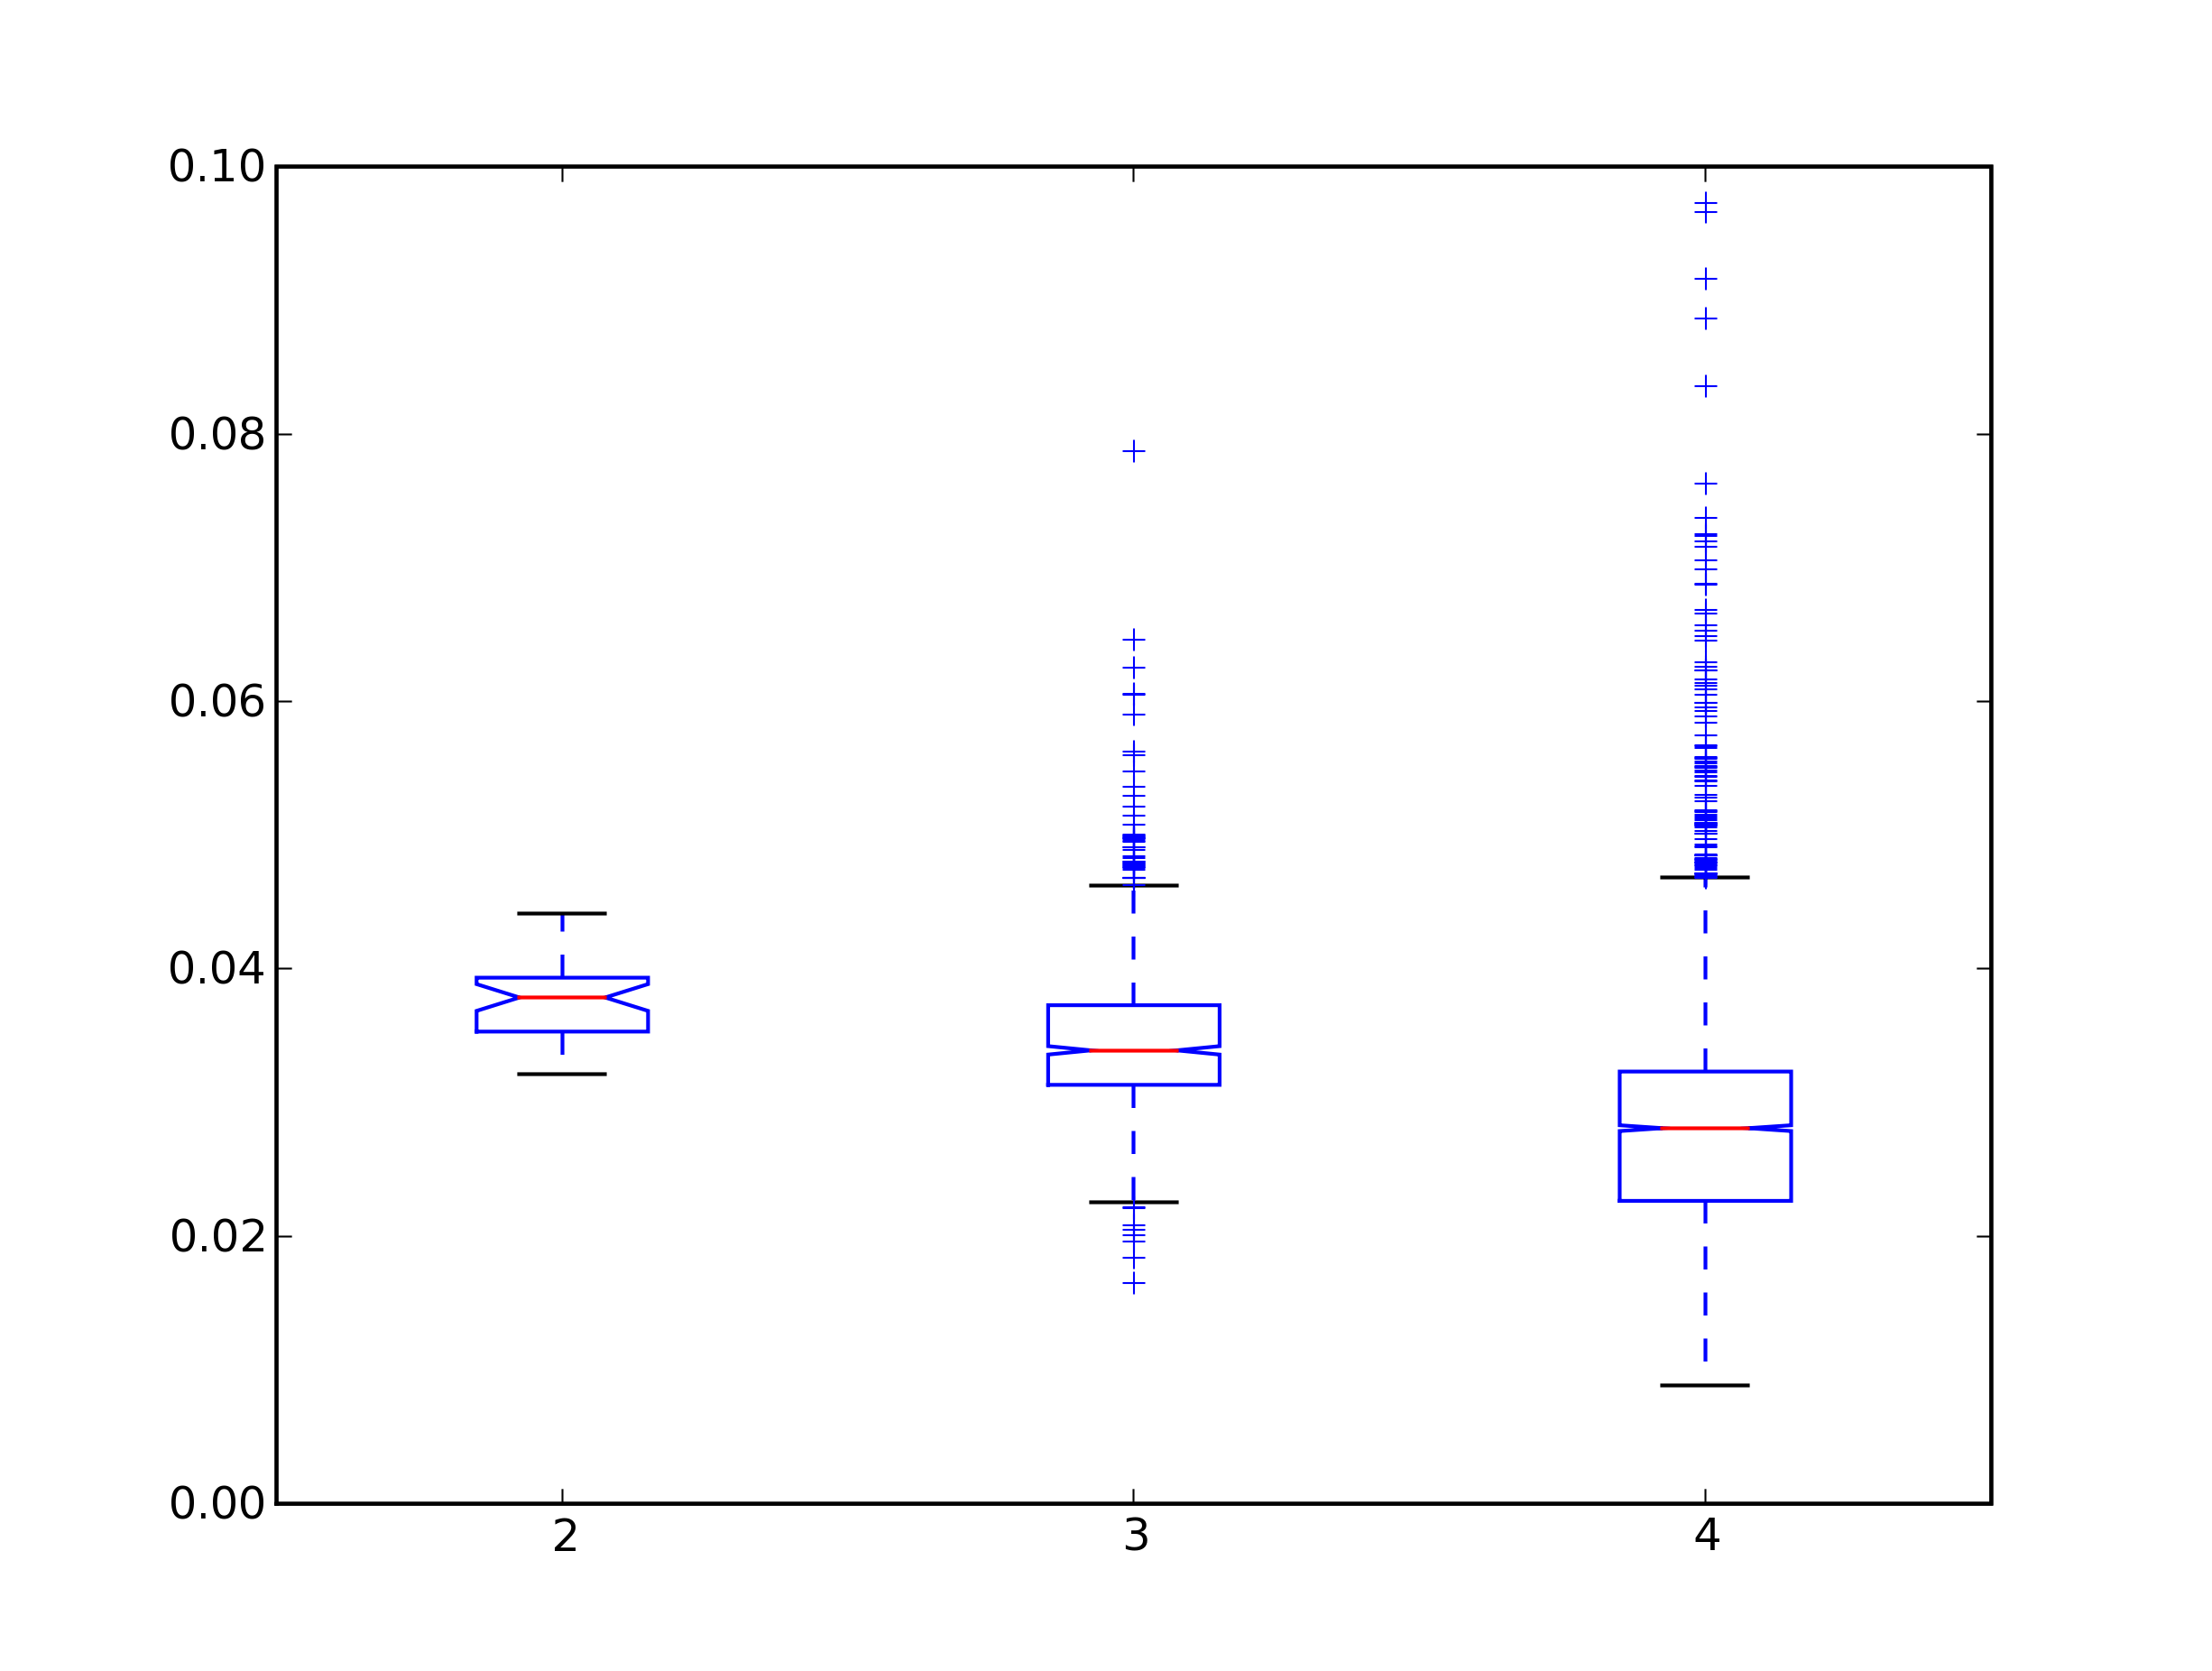
\includegraphics[width=.45\linewidth]{rook_iv_box.png}
}
\subfigure[Hexagonal Topology]{
  \label{boxplot:hex}
  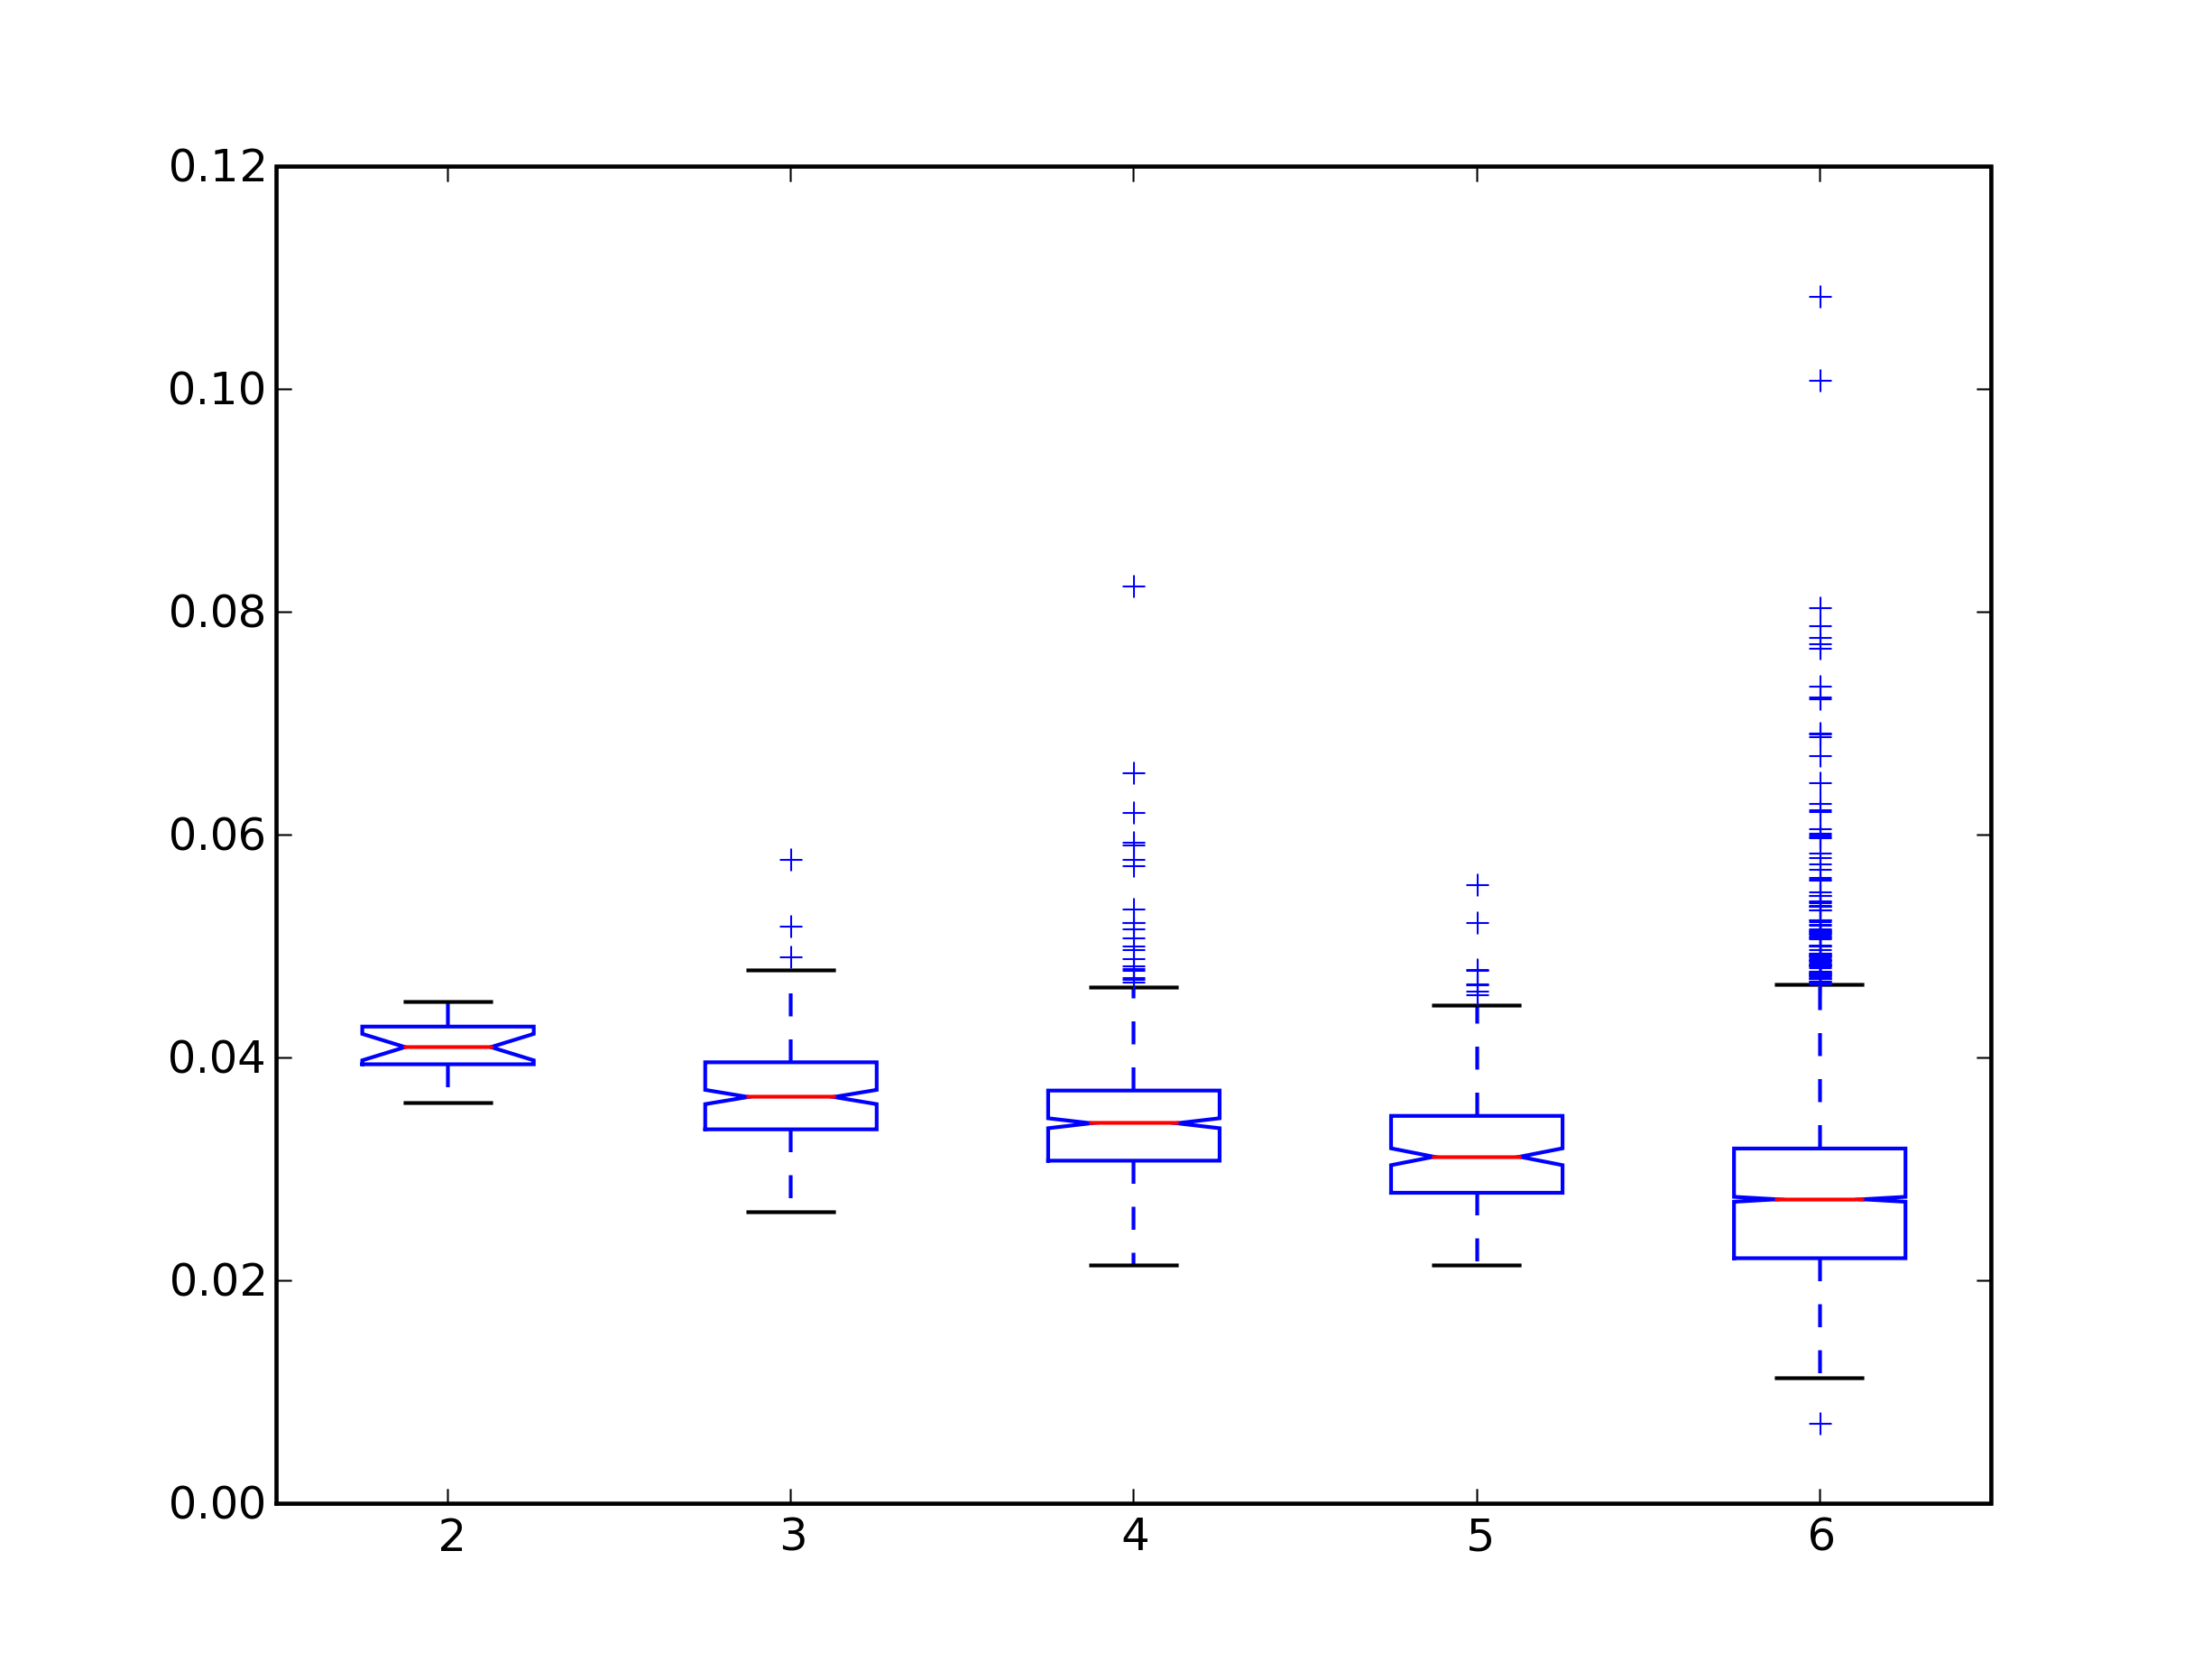
\includegraphics[width=.45\linewidth]{hex_iv_box.png}
}
\subfigure[Spherical Topology]{
  \label{boxplot:graph}
  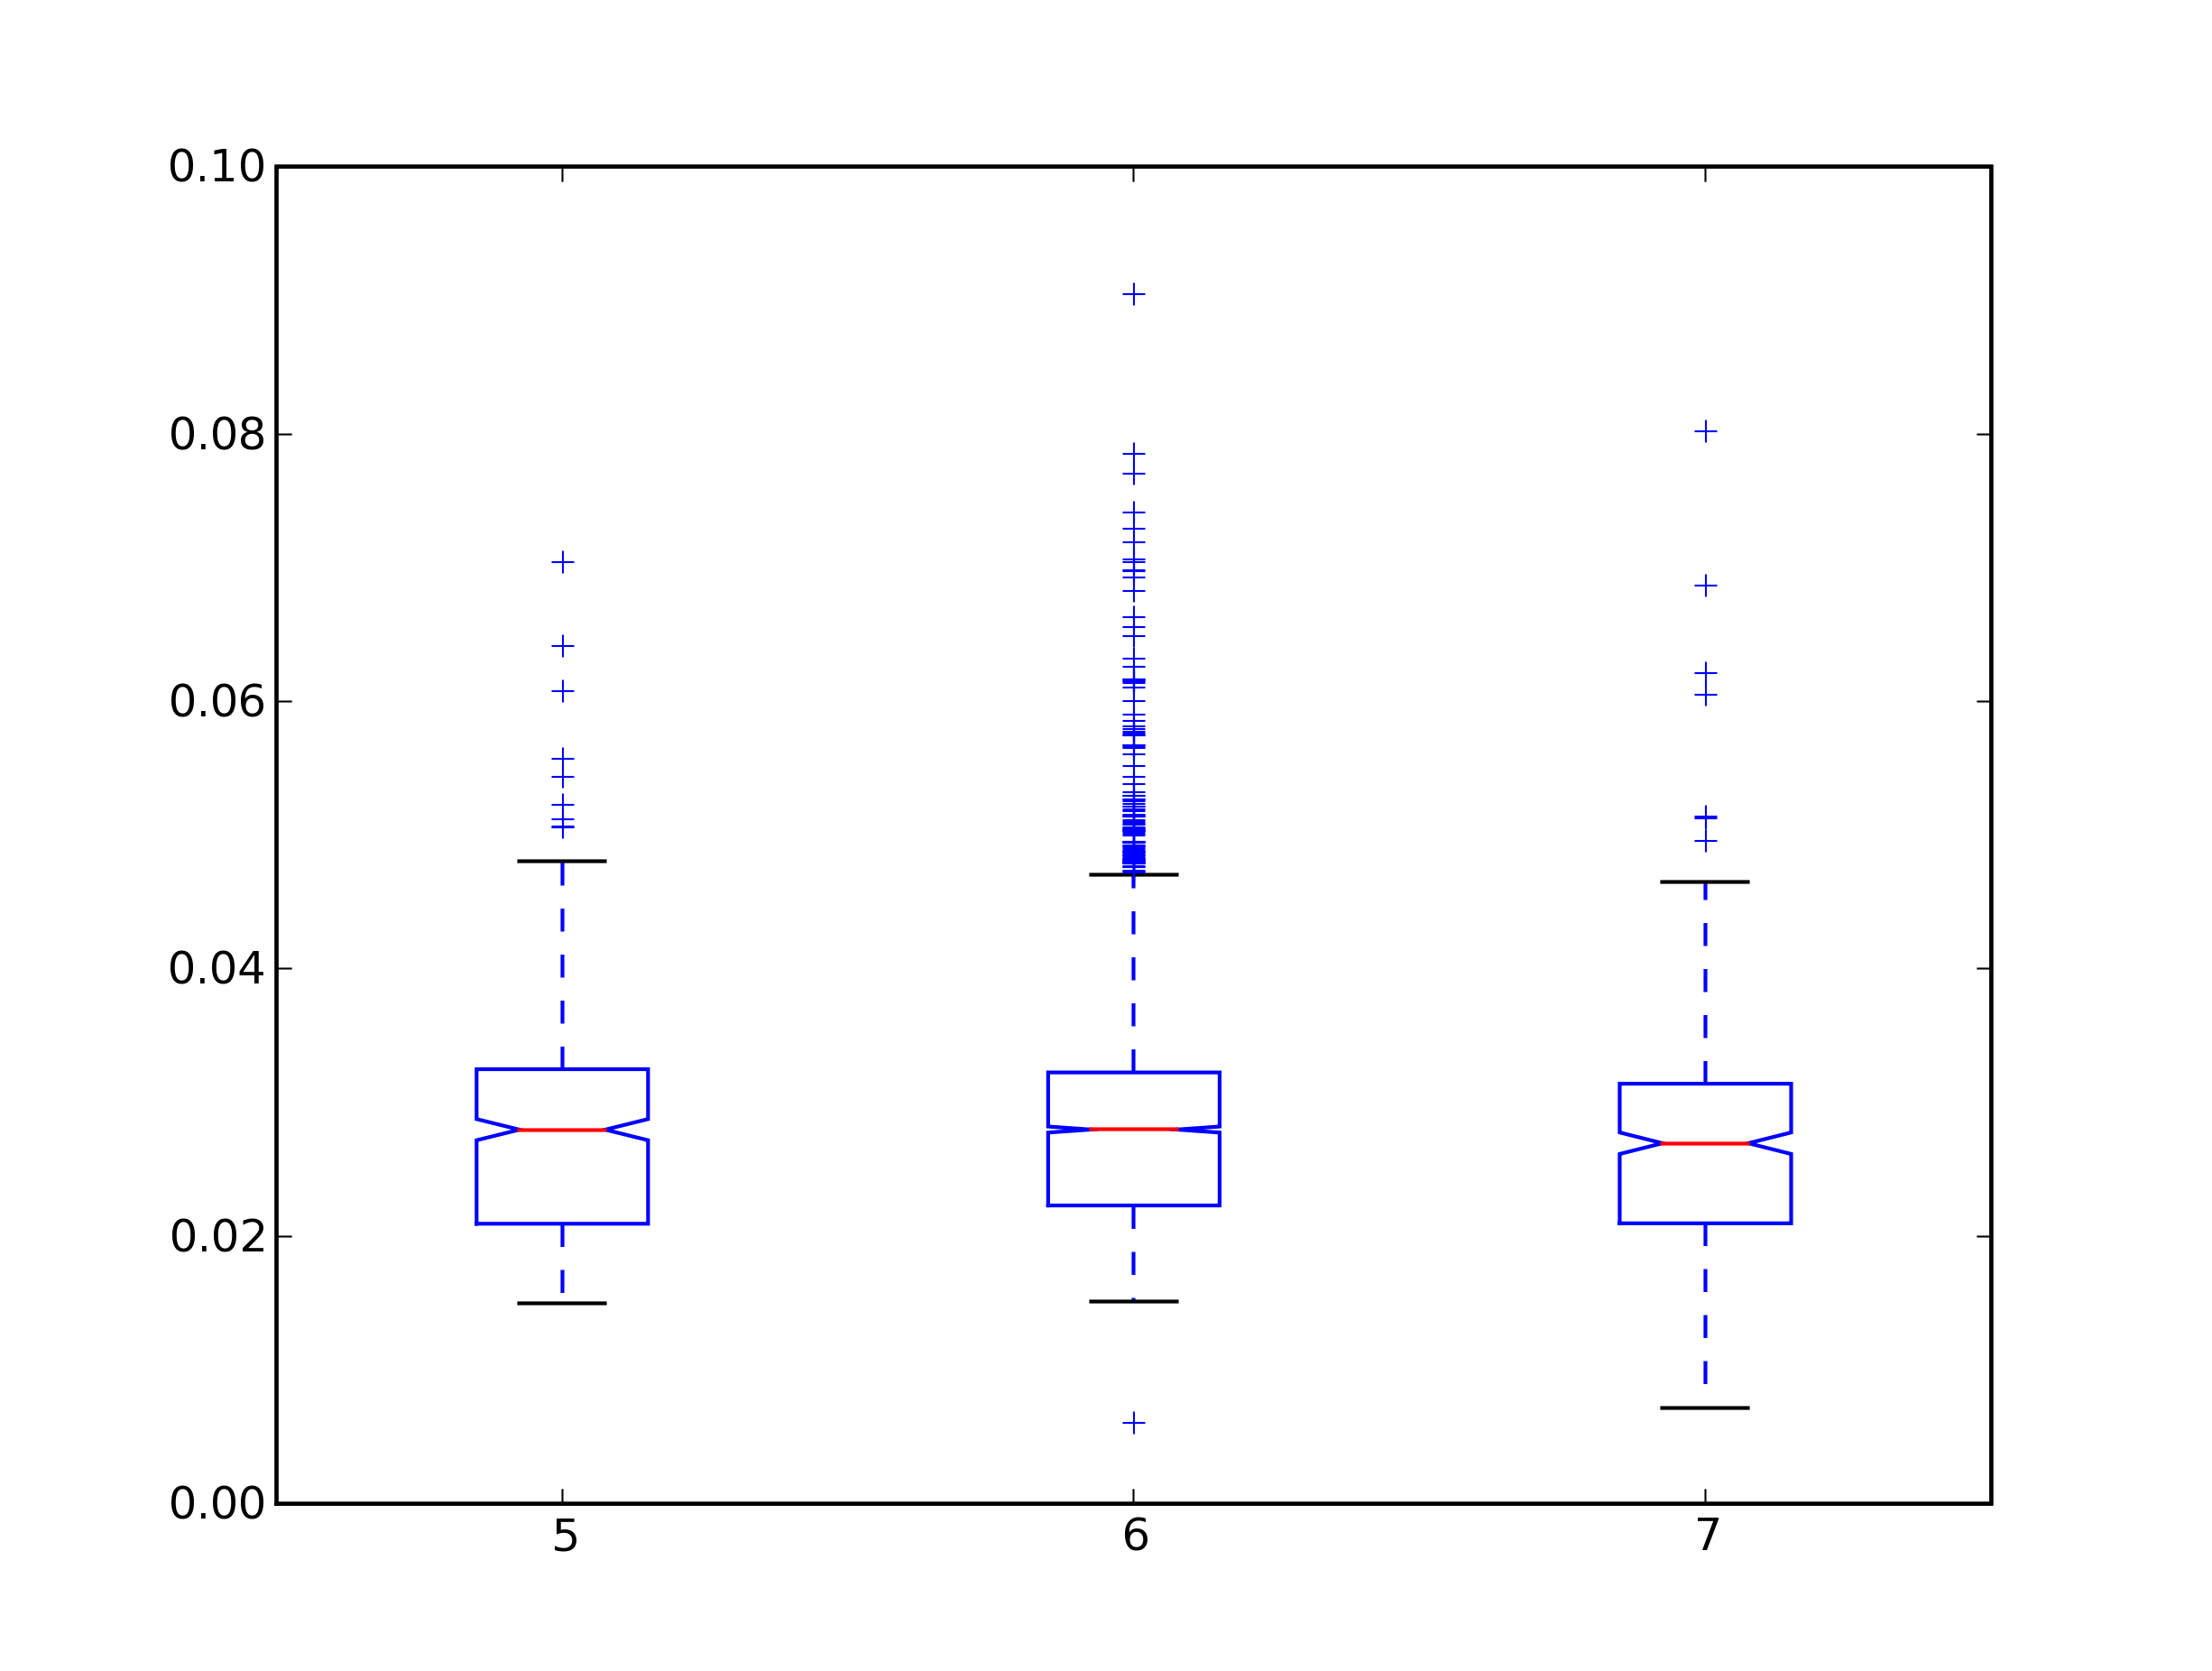
\includegraphics[width=.45\linewidth]{graph_iv_box.png}
}
\subfigure[Geodesic Sphere Topology]{
  \label{boxplot:geodesic}
  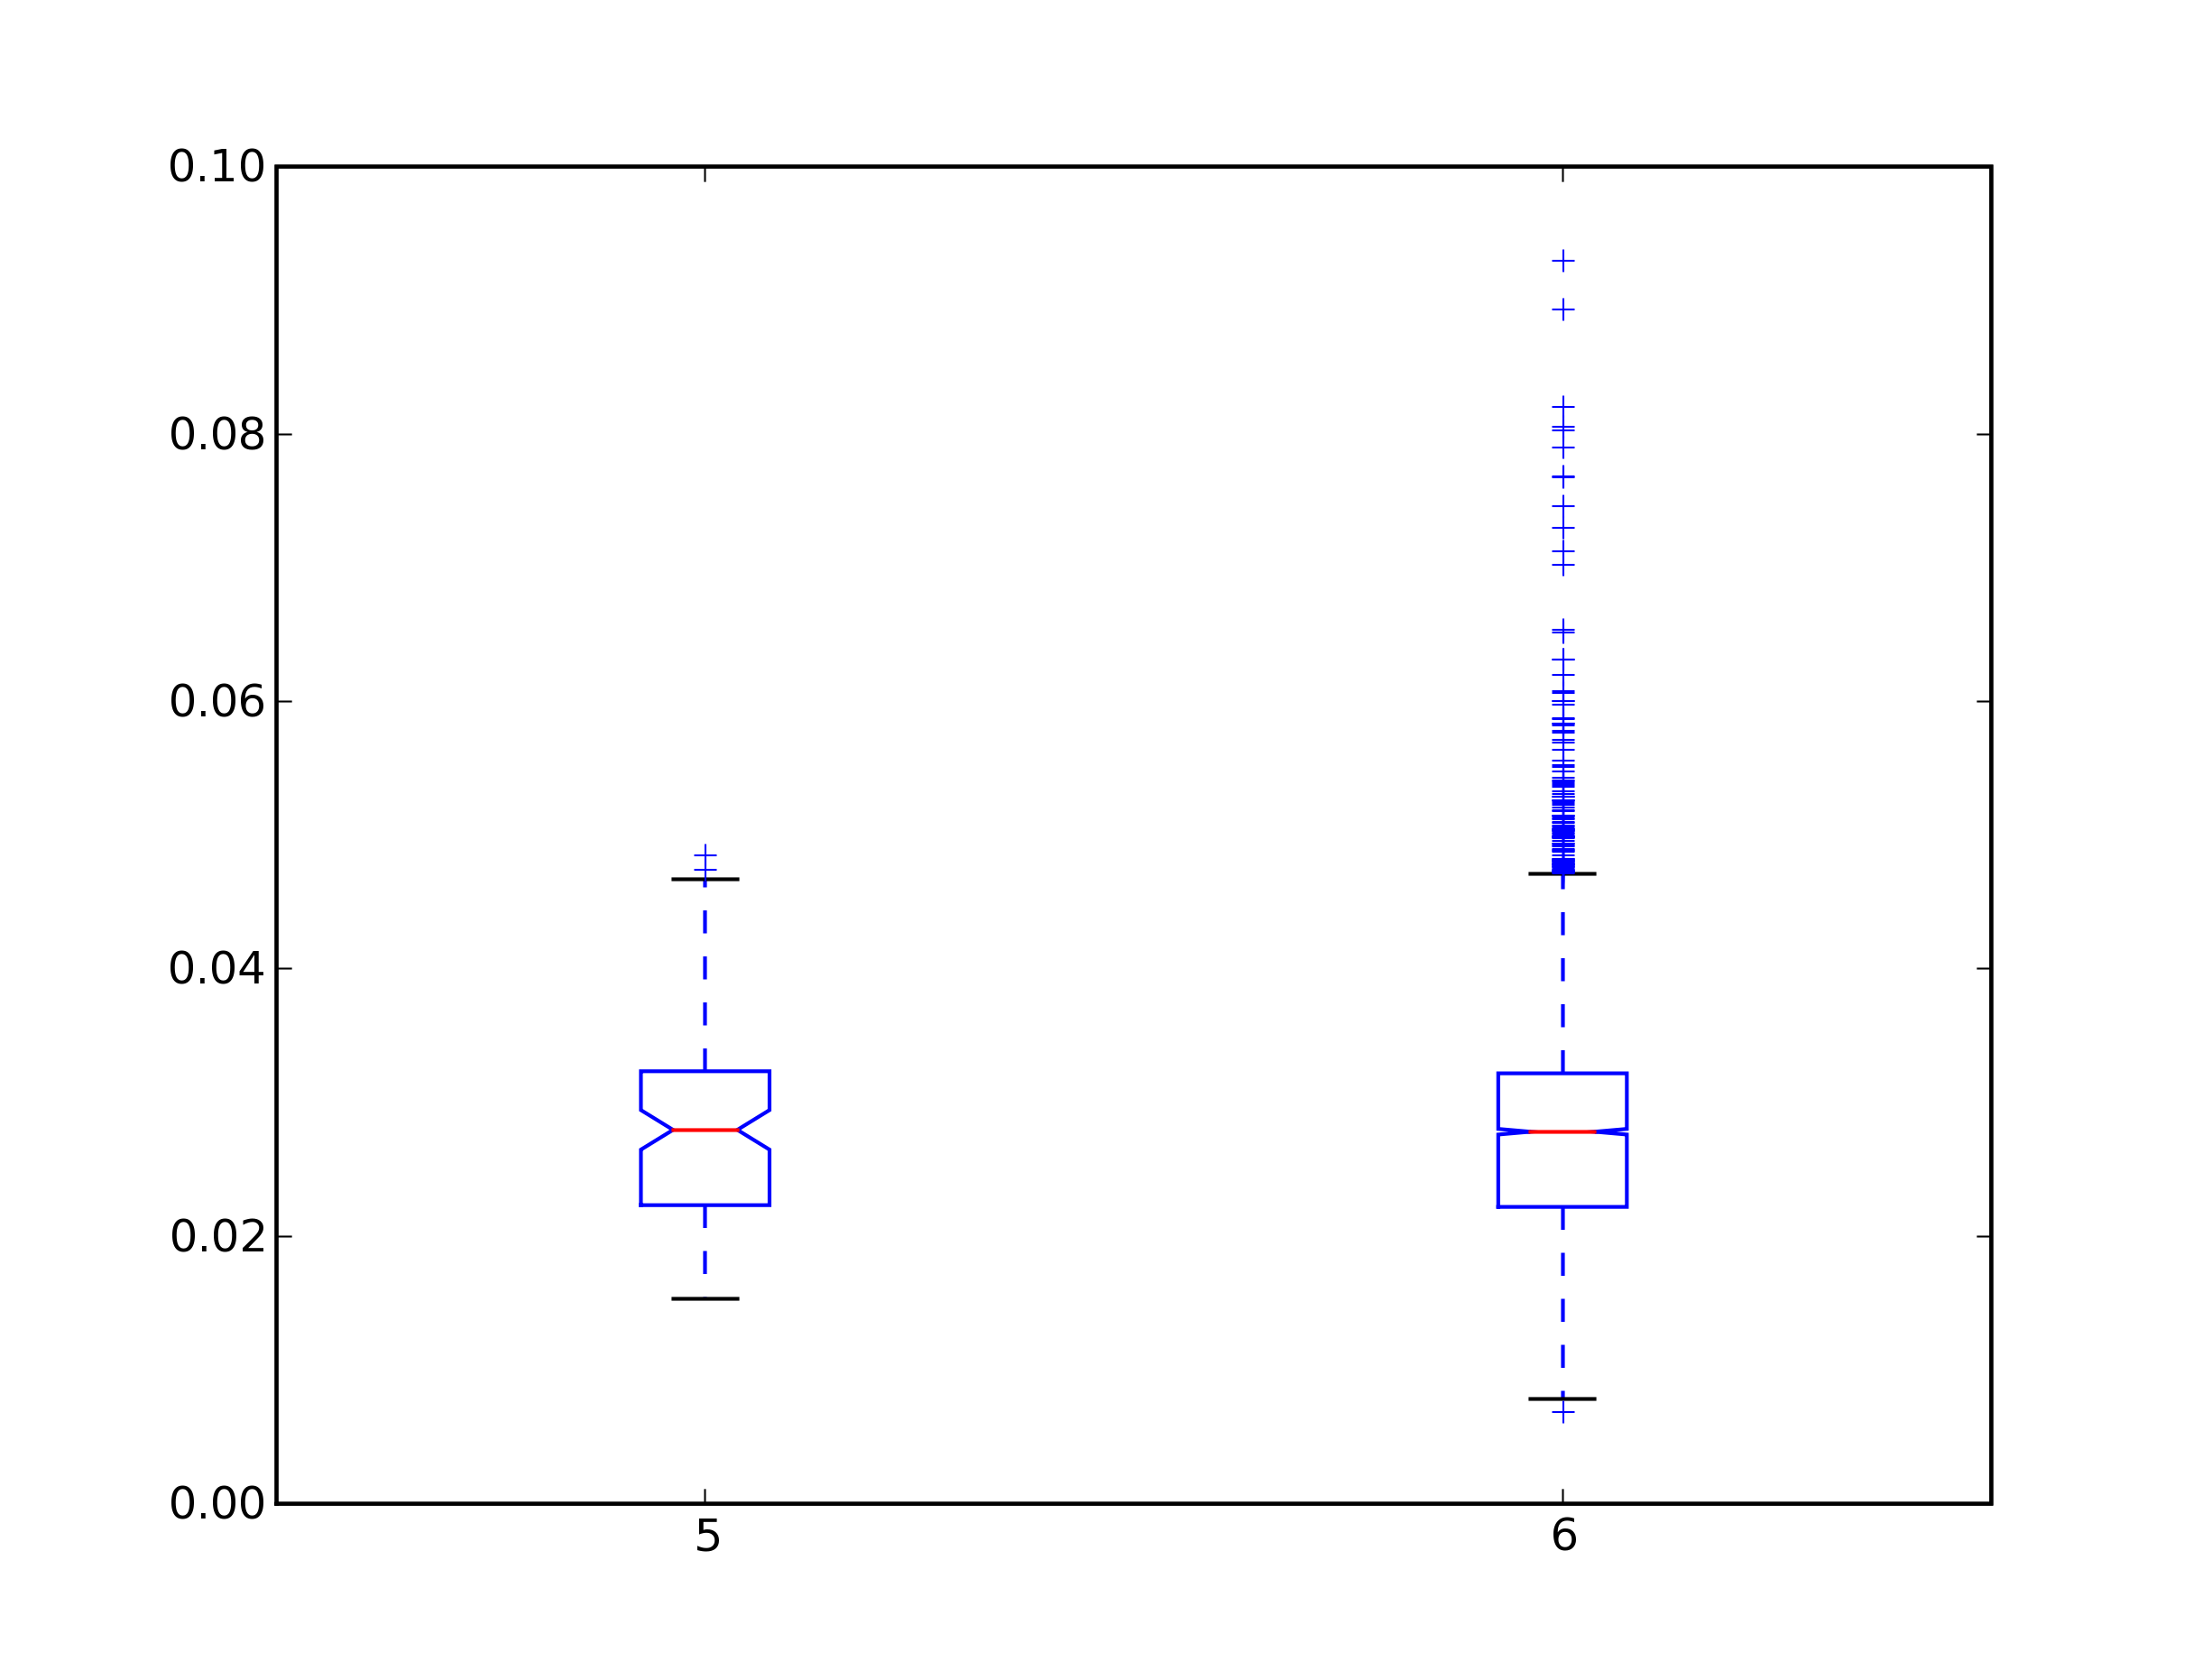
\includegraphics[width=.45\linewidth]{geodesic_iv_box.png}
}
\caption{This shows 4 box plots, each representing one group of neurons in a set
of SOMs trained with the same parameters.}
\label{boxplot}
\end{figure}

%I suspect a better measure would be to use the minimum number of steps for a
%given nueron to reach every other neuron on the network.  This would vary
%significantly on the rook and hexagon topolgoies, but not very much in the
%spherical topologies.

%\begin{landscape}
\begin{table}[hbt]
\centering
%\scriptsize
\begin{minipage}{\textwidth}
\caption{Mean IV and Var(IV) grouped by a neurons degree for each topology}
\label{meanvar1}
\begin{tabular}{|c||cc|cc|cc|cc|}
\hline
\textbf{Degree} & \multicolumn{2}{c|}{\textbf{Geodesic}} &
\multicolumn{2}{c|}{\textbf{Spherical}} &
\multicolumn{2}{c|}{\textbf{Hexagonal}} &
\multicolumn{2}{c|}{\textbf{Rectangular}} \\
\hline
& N & Mean (Var) & N & Mean (Var) & N & Mean (Var) & N & Mean (Var) \\
\hline
2&&&&& 20& 0.0409 (5.66E-06)& 40& 0.0378 (7.59E-06)\\ 
3&&&&& 218& 0.0371 (2.18E-05)& 880& 0.0348 (3.59E-05)\\ 
4&&&&& 489& 0.0347 (4.05E-05)& 4926& 0.0284 (6.28E-05)\\ 
5& 113& 0.0283 (5.28E-05)& 526& 0.0279 (6.43E-05)& 206& 0.0319 (3.50E-05)&&\\ 
6& 5598& 0.0281 (6.05E-05)& 4758& 0.0282 (6.05E-05)& 4954& 0.0278
(6.09E-05)&&\\ 
7&&& 417& 0.0273 (6.65E-05)&&&&\\ 
\hline
\end{tabular} \end{minipage} \end{table}
%\end{landscape}



%\subsection{Restate the Questions}
%\textbf{Objective}, Compare the internal variance of observations captured by a given
%neuron to that neuron's first-order neighborhood size.
%\textbf{Question}, Does the internal variance of a neuron decrease as its first-order
%neighborhood size, or degree, increases?


\begin{table}[hbt]
\centering
\caption{These tables show the difference in mean IV between each group of
neurons grouped by their degree, delta (significance),
t=9999, *** = 99\%, ** = 95\%, * = 90\%}
\label{rlt}


  \subtable[Rectangular Topology]{
    \label{rlt:rook}
    \begin{tabular}{|c||c|c|c|}
    \hline
    Degree&2&3&4\\\hline
    \hline
    2 & (0.000008) & \textbf{0.002000} & \textbf{0.001000}\\\hline
    3 & 0.002969 & (0.000036) & \textbf{0.001000}\\\hline
    4 & 0.009364 & 0.006396 & (0.000063)\\\hline
    \end{tabular}
  }

  \subtable[Hexagonal Topology]{
    \label{rlt:hex}
    \begin{tabular}{|c||c|c|c|c|c|}
    \hline
    Degree&2&3&4&5&6\\ \hline
    \hline
    2 & (0.000006) & \textbf{0.001000} & \textbf{0.001000} & \textbf{0.001000} & \textbf{0.001000}\\\hline
    3 & 0.003810 & (0.000022) & \textbf{0.001000} & \textbf{0.001000} & \textbf{0.001000}\\\hline
    4 & 0.006253 & 0.002443 & (0.000040) & \textbf{0.001000} & \textbf{0.001000}\\\hline
    5 & 0.009008 & 0.005197 & 0.002755 & (0.000035) & \textbf{0.001000}\\\hline
    6 & 0.013067 & 0.009257 & 0.006814 & 0.004059 & (0.000061)\\\hline
    \end{tabular}
  }

  \subtable[Spherical Topology]{
    \label{rlt:graph}
    \begin{tabular}{|c||c|c|c|}
    \hline	
    Degree&5&6&7\\ \hline
    \hline
    5 & (0.000064) & 0.487000 & 0.199000\\\hline
    6 & 0.000250 & (0.000060) & \textbf{0.023000}\\\hline
    7 & 0.000674 & 0.000924 & (0.000067)\\\hline
    \end{tabular}
  }

  \subtable[Geodesic Topology]{
    \label{rlt:geodesic}
    \begin{tabular}{|c||c|c|}
    \hline
    Degree&5&6\\ \hline
    \hline
    5 & (0.000053) & 0.756000\\\hline
    6 & 0.000203 & (0.000060)\\\hline
    \end{tabular}
  }
\end{table}

\section{Internal variance vs. centrality}
\label{rdq2}
Above we saw that changes in a neuron's degree was related to changes in
internal variance in topologies with edges, but not in the two sphere based
topologies. The next step is to see if internal variance changes between
topologies.  To do this we will first order out topologies by a summary
measure of the network centrality.  A node's centrality can be thought of as a
measure of it's importance to the rest of the network. Above we used the most
common measure of centrality, which is a node's degree.  For this diagnostic
we'll take the variance of those degrees as a summary measure.  This should
tell us how regular the overall network is.  These variances and the sorting
of our topologies is shown in table \ref{vardeg}.

\begin{table}[hbt]
\centering
\caption{This table shows how our topologies will be sorted based on the
variance in degrees of the topology's nodes}
\label{vardeg}
\begin{tabular}{|c|c|c|c|}
\hline
Topology & Var of Degree & MeanIV (VarIV)\\
\hline
Geodesic & 0.0183 & 0.0874 (0.0009)\\
Rectangular & 0.1457 & 0.0890 (0.0010)\\
Spherical & 0.1648 & 0.0879 (0.0010)\\
Hexagonal & 0.6283 & 0.0885 (0.0010)\\
\hline
\end{tabular}
\end{table}

Figure \ref{q2boxplot} shows the distribution on internal variance
measurements for each of our topologies.  It is interesting to note that
they all appear to be very similar. We test the difference in means for
each of these using the same method of random labeling that was applied in the
previous diagnostic. The results are displayed in table \ref{rlt:all}. Table
\ref{rlt:allV} shows the result of testing for a difference in variance
between each topology.  It was expected that the mean and variance of IV would
increase in more irregular topologies.  These result general do not support
that hypothesis. This may suggest that the mean and variance of IV are not
appropriate summary measures.

\begin{figure}[hbt]
\centering
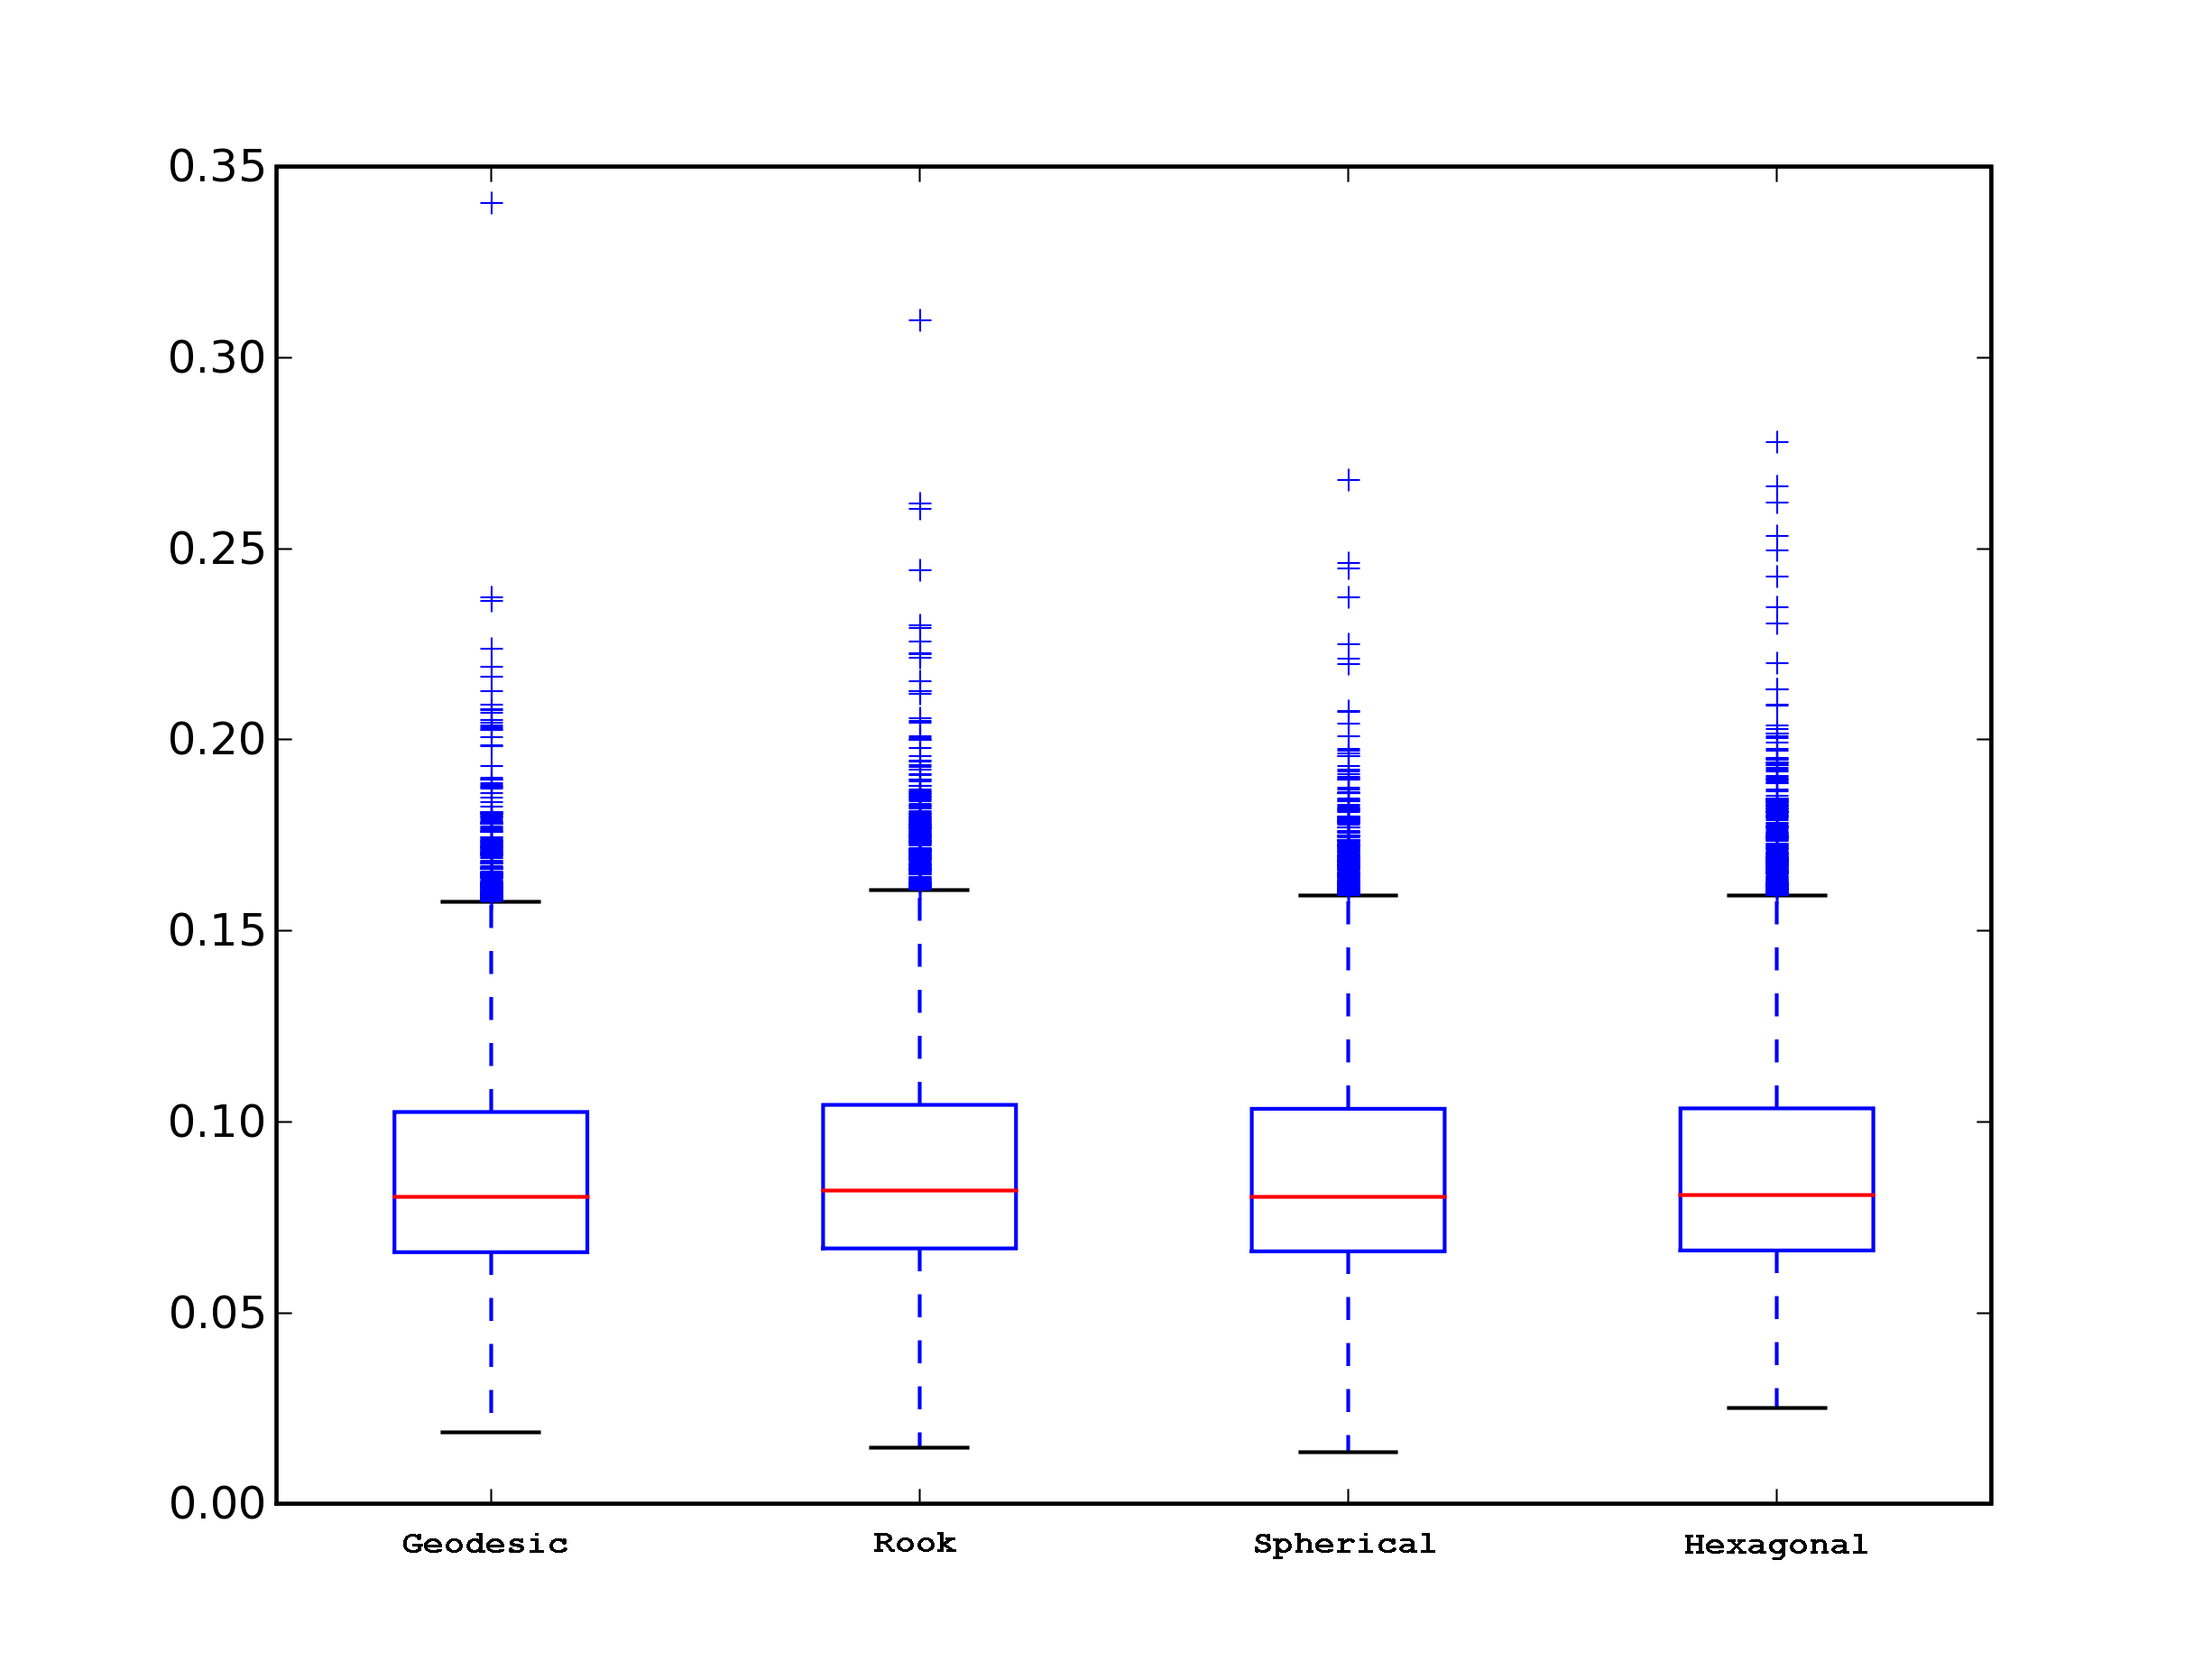
\includegraphics[width=\linewidth]{q2boxplot.png}
\caption{These box plots show the distribution of internal variance measurements
for each topology.}
\label{q2boxplot}
\end{figure}


\begin{table}[hbt]
  \centering
  \caption{These tables show the difference in means of the internal variance between each topology}
  \label{rlt:all}
  \begin{tabular}{|c||c|c|c|c|}
  \hline
  \textbf{Topology}&Geodesic &Rectangular	&Sphere			&Hexagonal		\\\hline
  \hline
  Geodesic	&& \textbf{0.0015} ***	& 0.0005		& \textbf{0.0010} *	\\\hline
  Rectangular		&& 			& \textbf{0.0011} *	& 0.0005		\\\hline
  Sphere	&& 			& 			& 0.0005 		\\\hline
  Hexagonal 	&& 			& 			&			\\\hline
  \end{tabular}
  \end{table}




\begin{table}[hbt]
  \centering
  \caption{These tables show the difference in variances of the internal variance between each topology}
  \label{rlt:allV}
  \begin{tabular}{|c||c|c|c|c|}
  \hline
  \textbf{Topology}&Geodesic &Rectangular	&Sphere			&Hexagonal		\\\hline
  \hline
  Geodesic	&& \textbf{0.0009} *	& 0.0003		& \textbf{0.0011} **	\\\hline
  Rectangular		&& 			& 0.0005		& 0.0002		\\\hline
  Sphere	&& 			& 			& 0.0007 		\\\hline
  Hexagonal 	&& 			& 			&			\\\hline
  \end{tabular}
  \end{table}



\section{Visualization of internal variance}
\label{rdq3}
In this section we will look at what information can be gained from
visualizing the SOM and its internal variance. The visualizations are created
with off the shelf GIS packages, namely ESRI's ArcGIS.  There are a number of
challenges which must be overcome before one can visualize the SOM.  To
visualize the rectangular and hexagonal topologies we simply need to create polygons
centered over each neuron.  The spherical and geodesic topologies are slightly
more complicated.  To create the polygons for these topologies we must first
compute the voronoi diagram on the surface of the sphere.  This is done using
``STRIPACK'', a software program created by \cite{Ranka97}.  The next problem
is that ArcGIS and other common GIS packages assume Cartesian distances.  They
can not handle polygons that cross the $180^{th}$ meridian.  To accommodate this we
must split each polygon at the $180^{th}$ meridian and draw it as two parts.  This
is done by checking each edge of each polygon to see if it crosses this
meridian, if it does we calculate its intersection with the meridian and split
the edge into two segments.

        Figure \ref{ten} shows cool stuff.





%\begin{figure}[hbt]
%	\centering
%	\includegraphics[width=\linewidth]{geo_poly.png}
%	\caption{This is a visualiation of the internal variance on the
%Geodesic SOM.}
%	\label{geopoly}
%\end{figure}

\begin{figure}[hbt]
\centering
\subfigure[Rectangular Topology]{
  \label{ten:rook}
  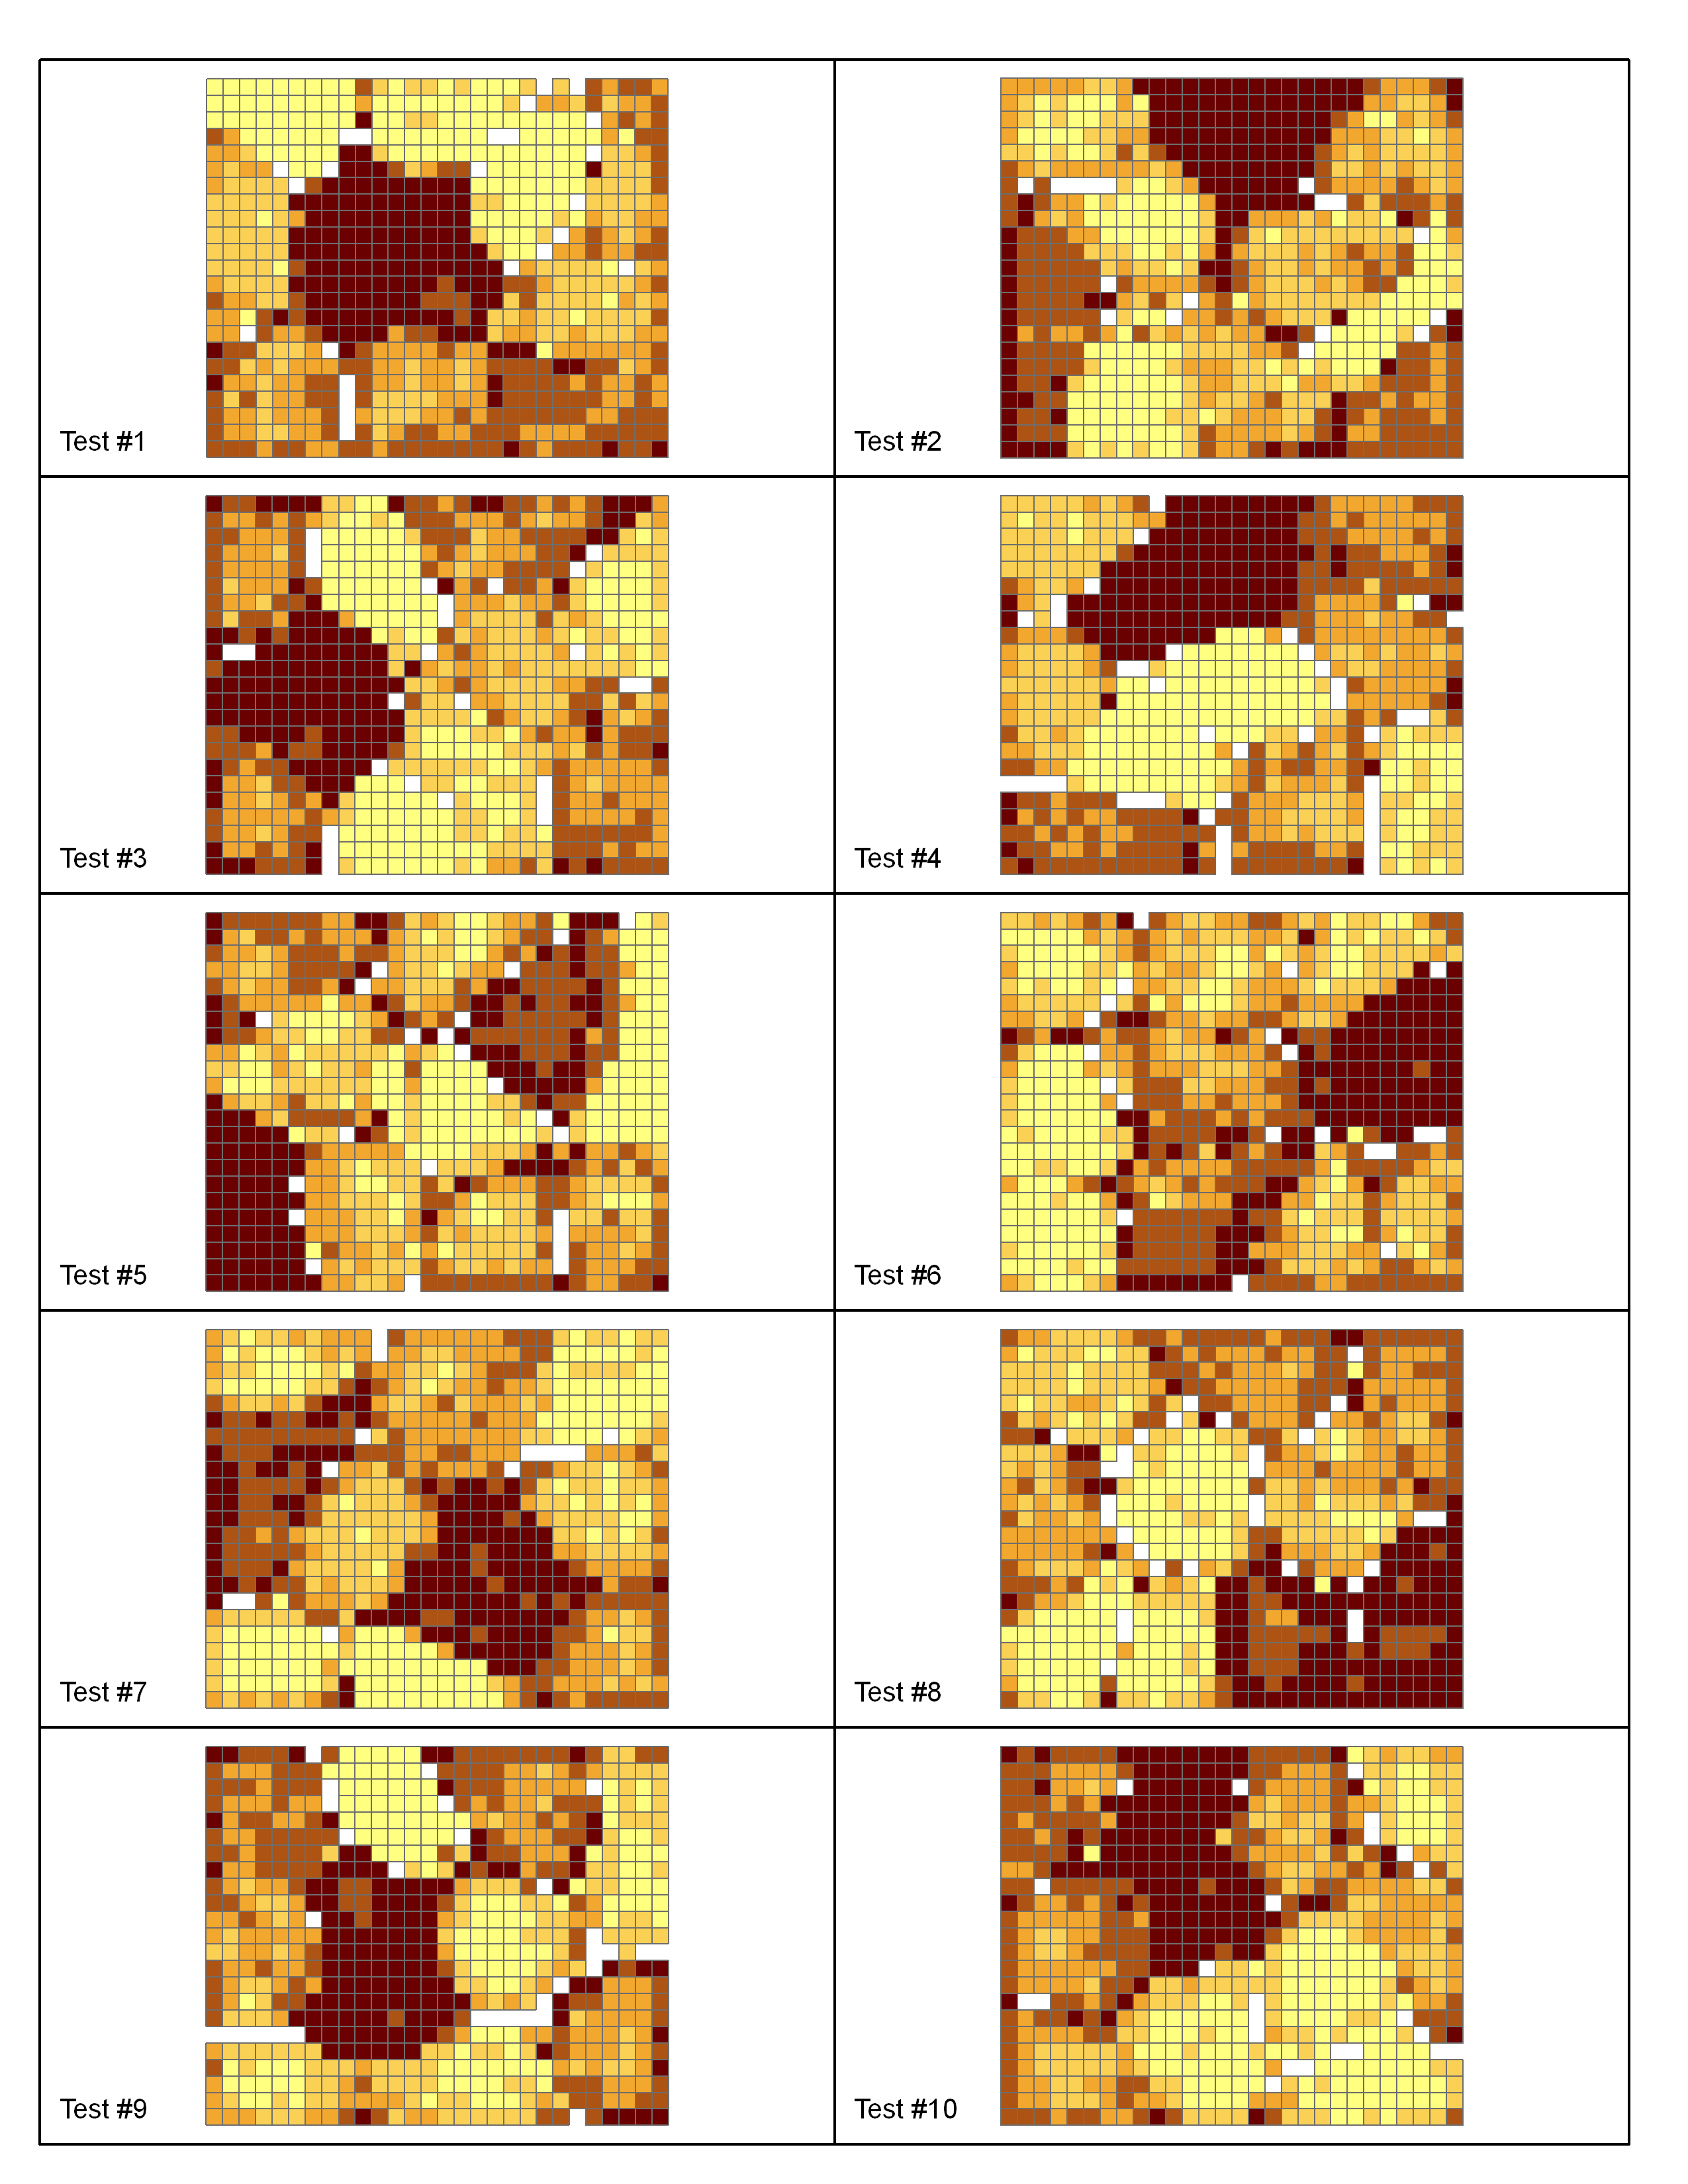
\includegraphics[width=.40\linewidth]{rook_10.png}
}
\subfigure[Hexagonal Topology]{
  \label{ten:hex}
  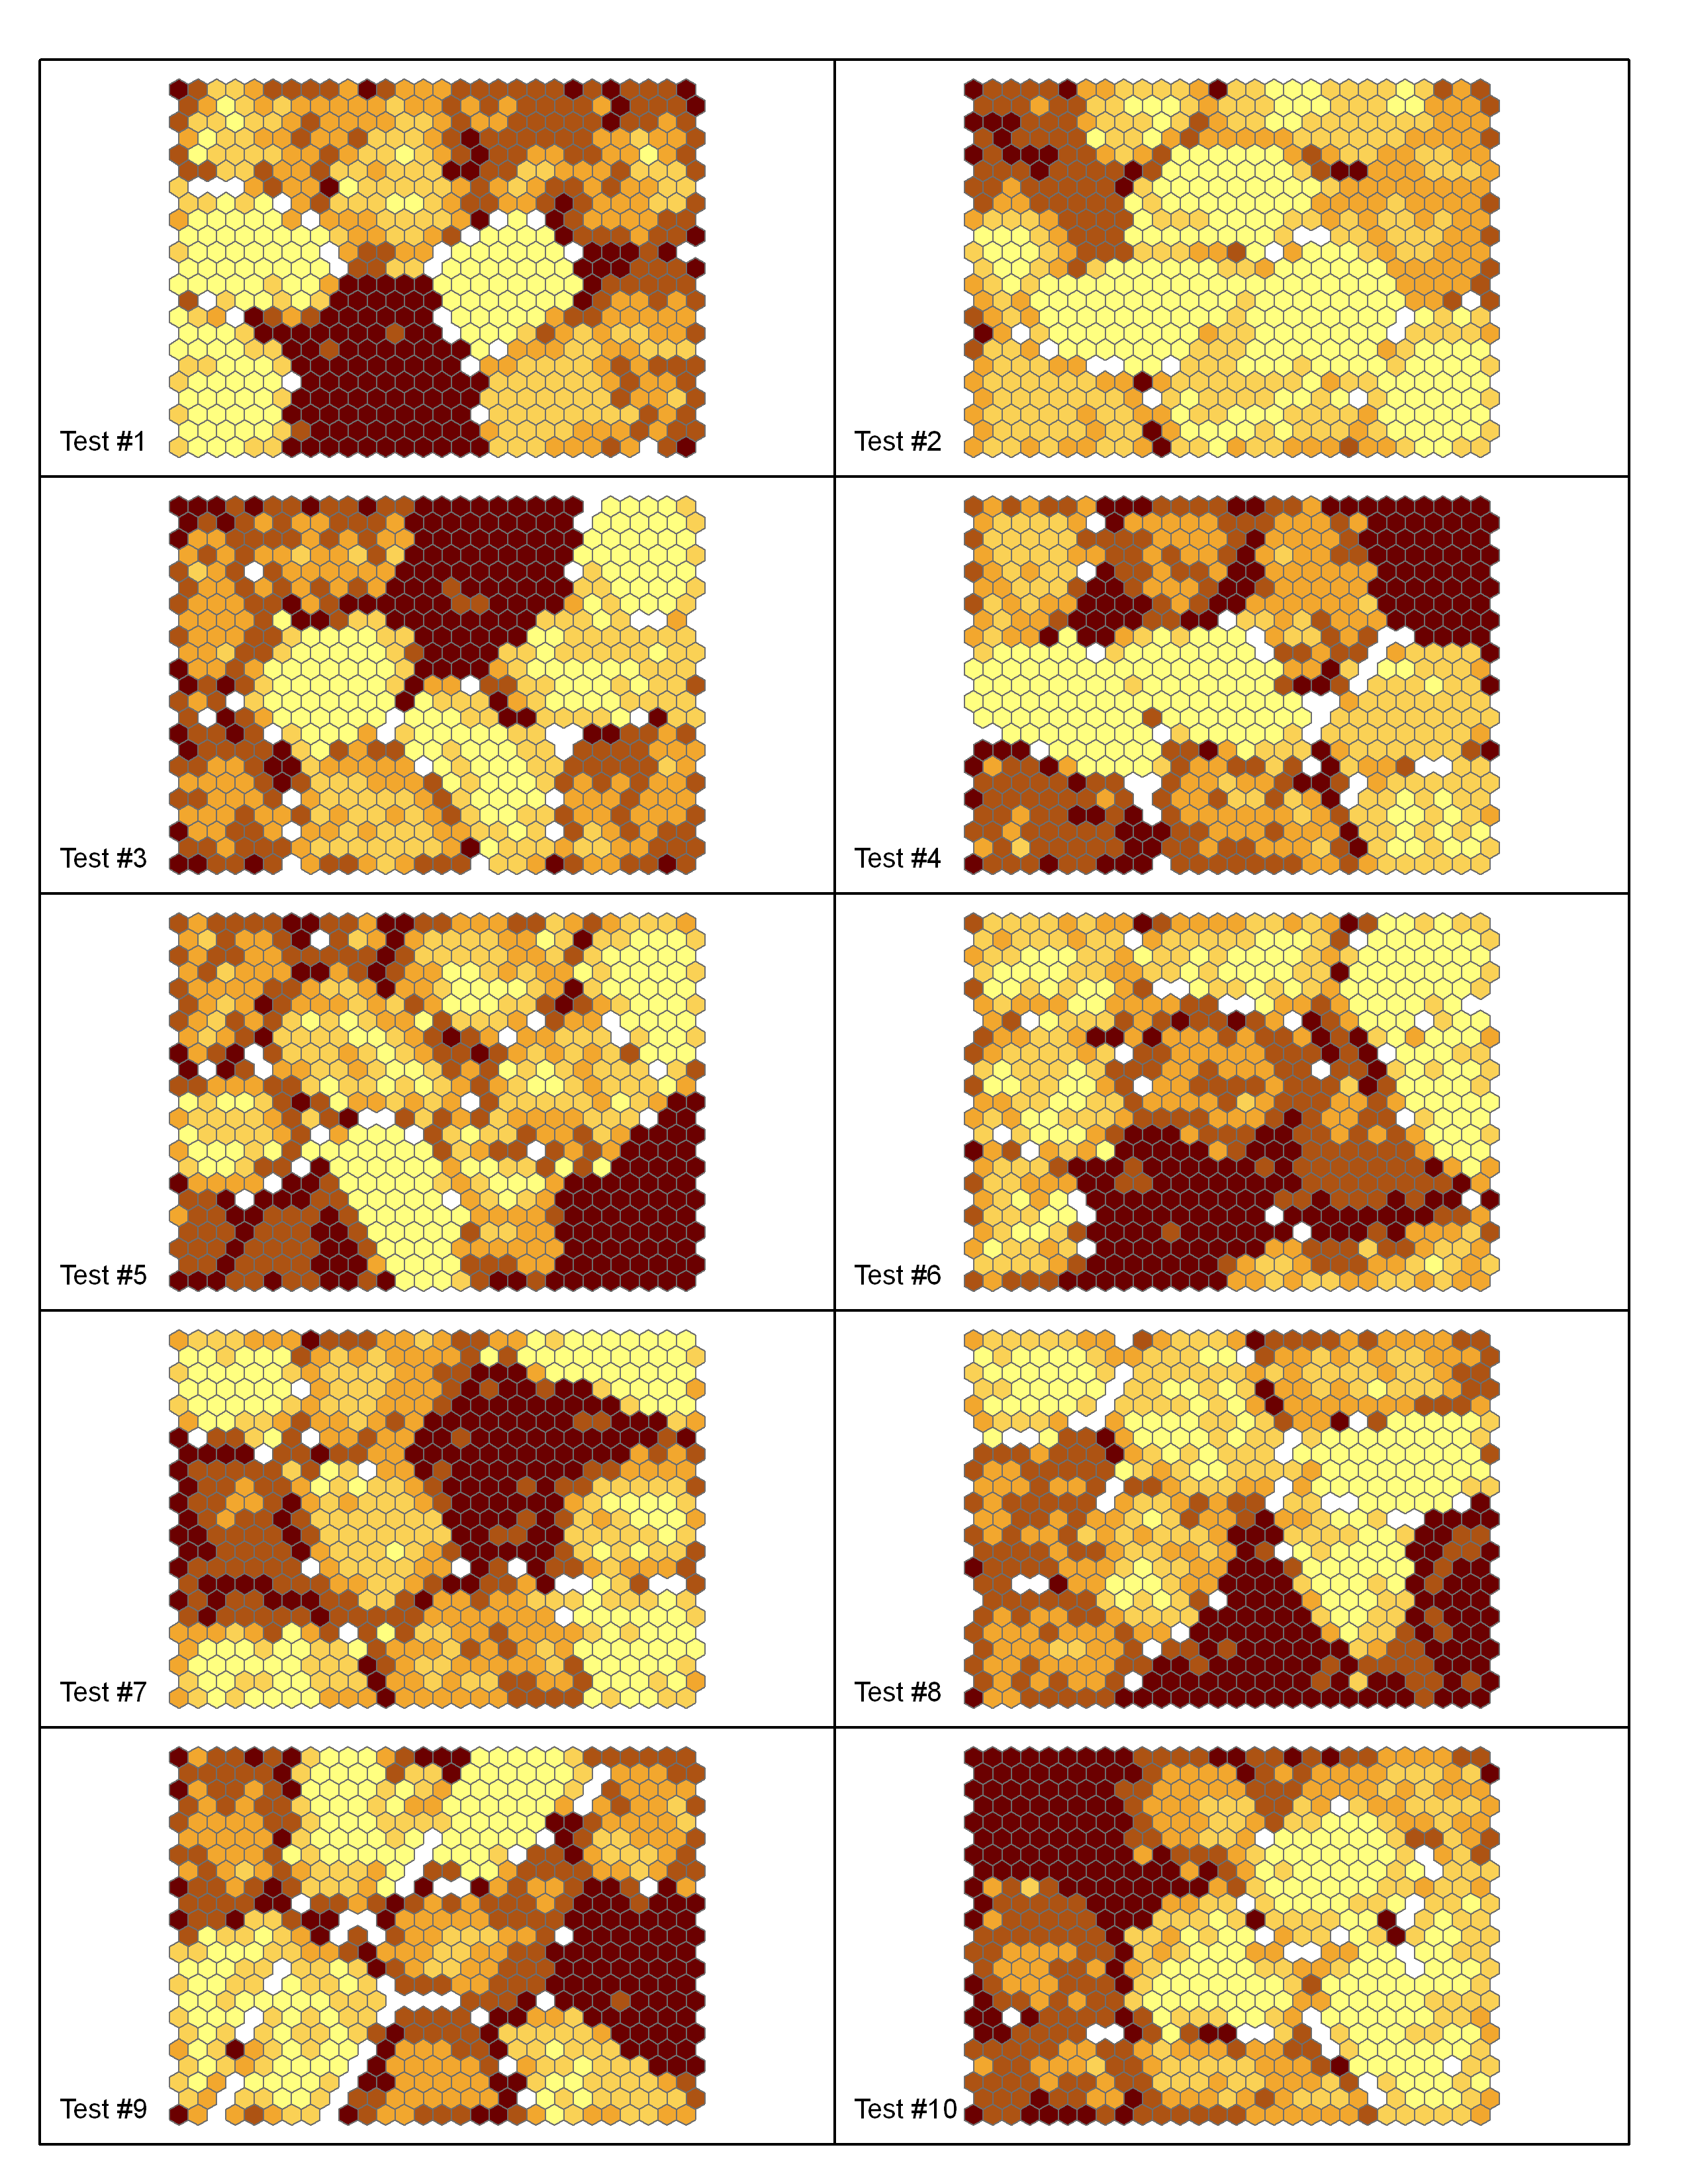
\includegraphics[width=.40\linewidth]{hex_10.png}
}
\subfigure[Spherical Topology]{
  \label{ten:graph}
  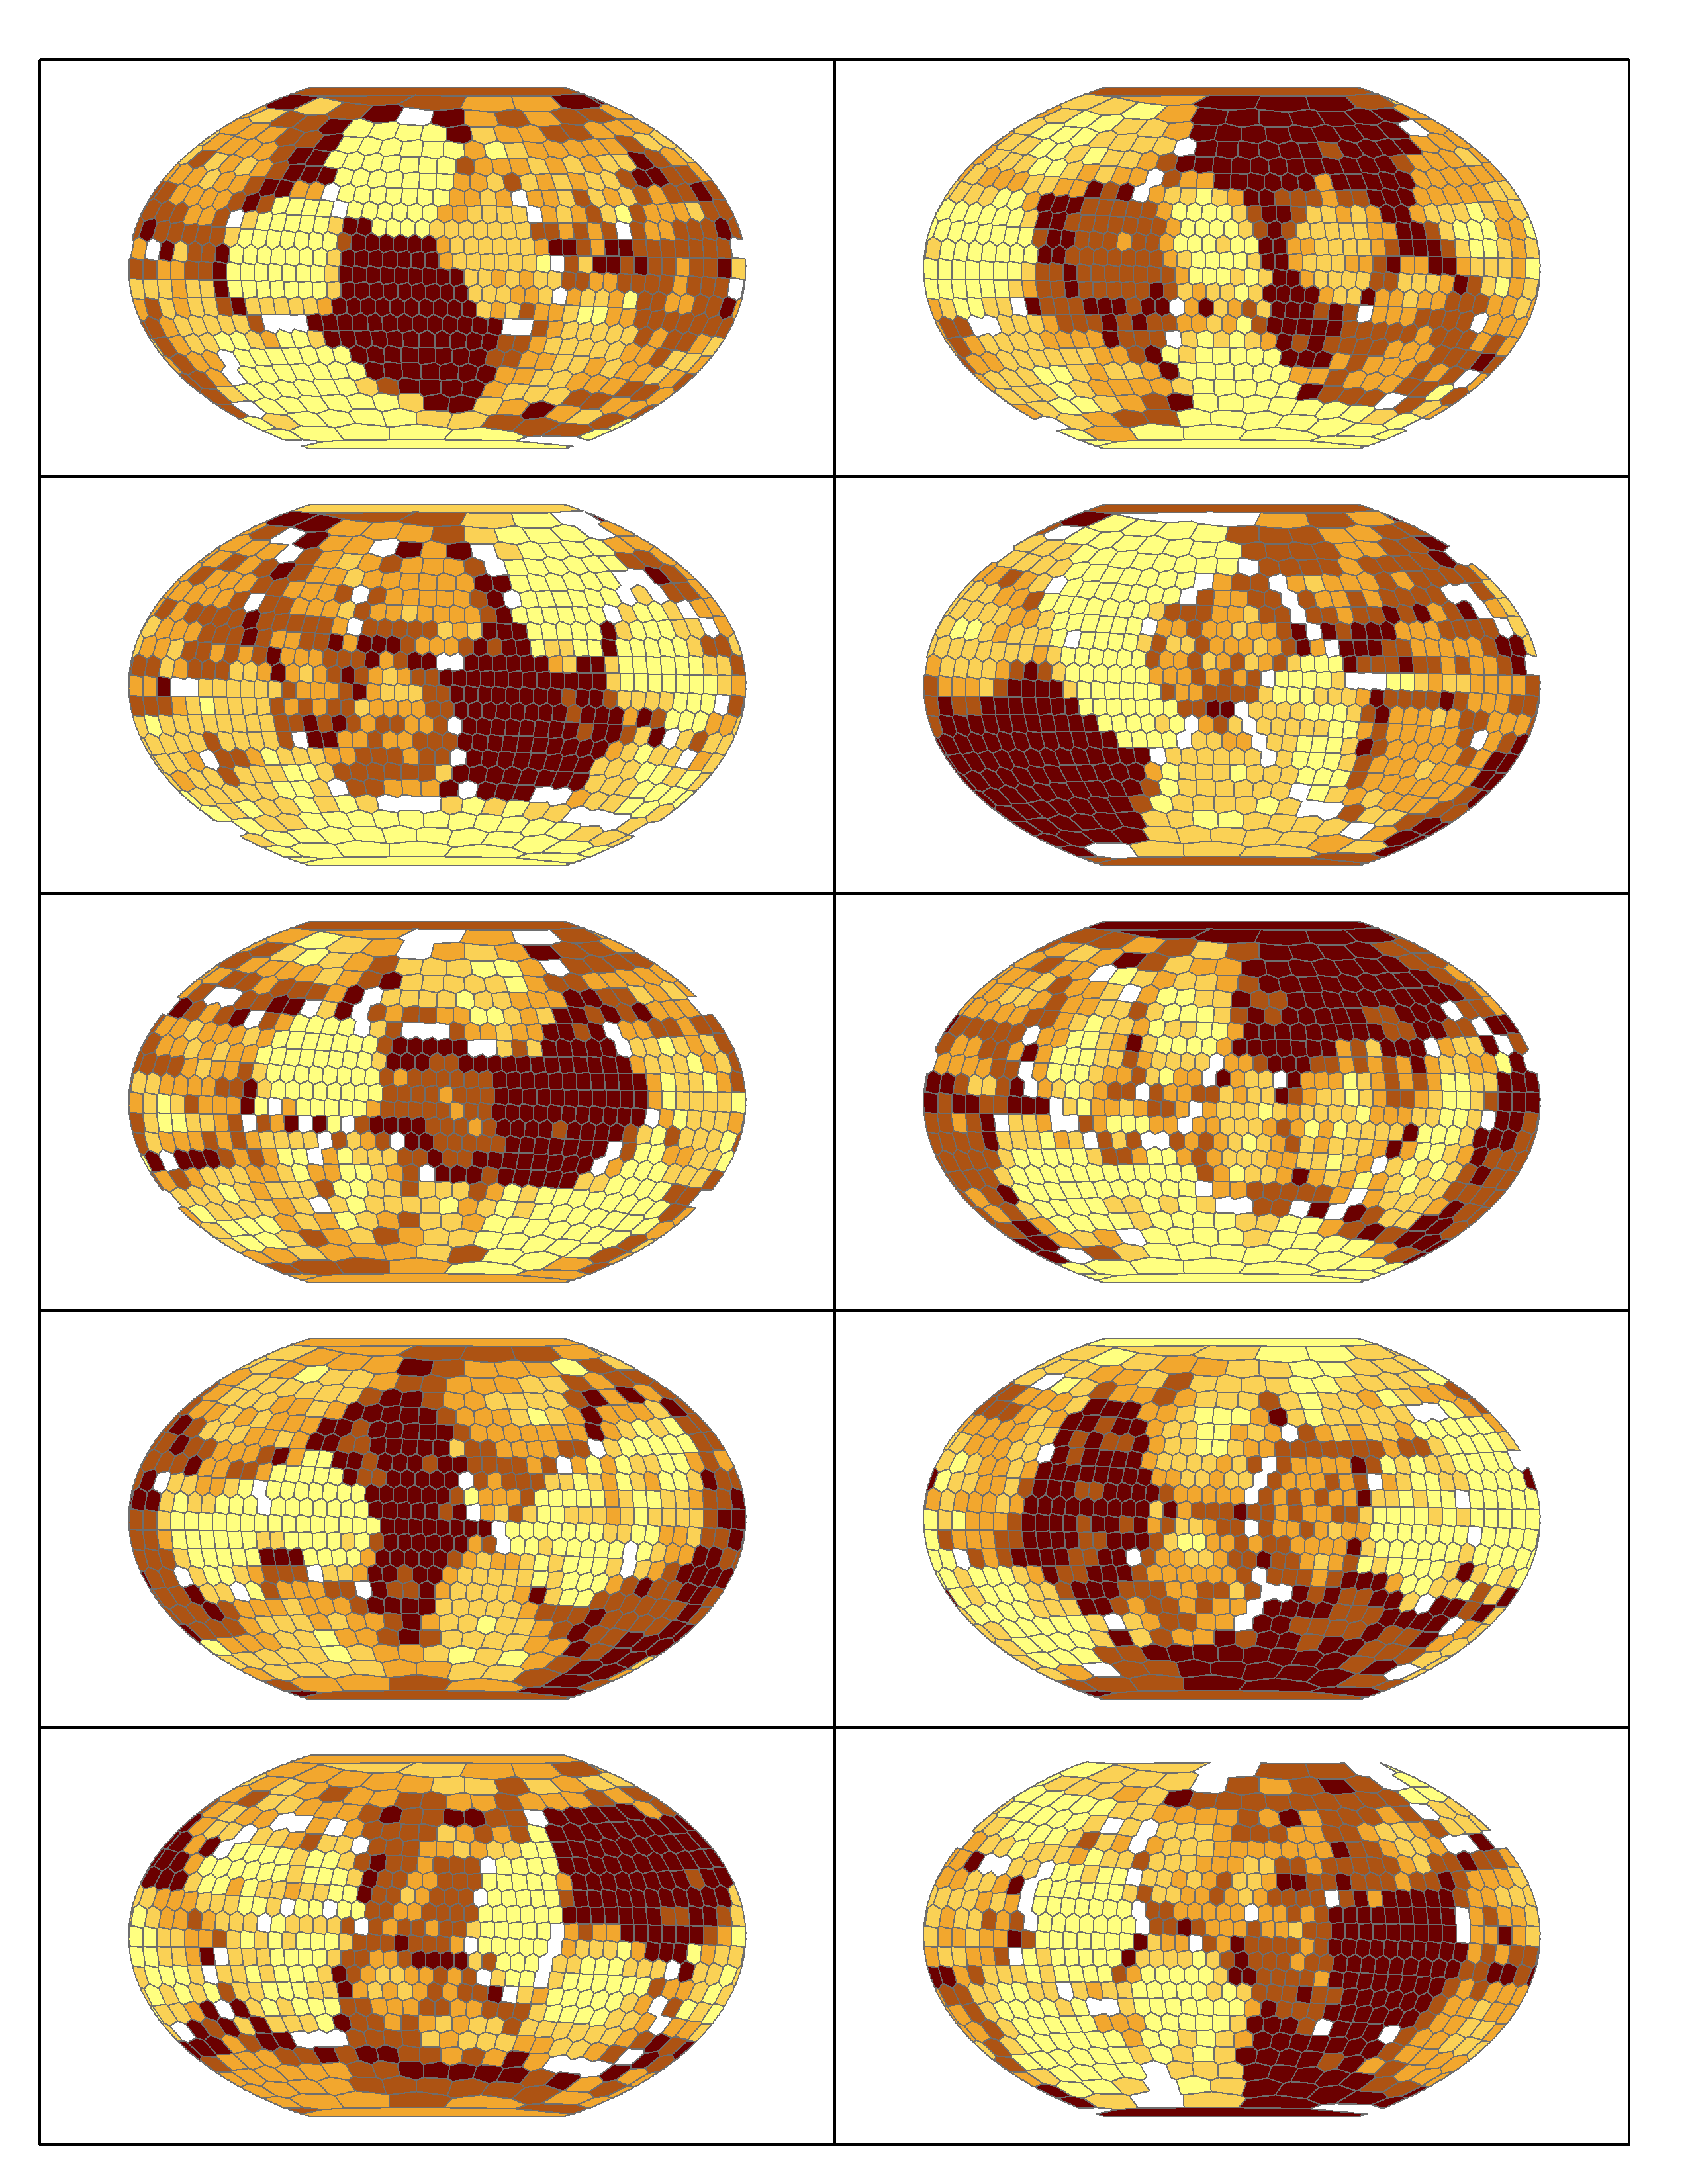
\includegraphics[width=.40\linewidth]{sphere_winkel.png}
}
\subfigure[Geodesic Sphere Topology]{
  \label{ten:geodesic}
  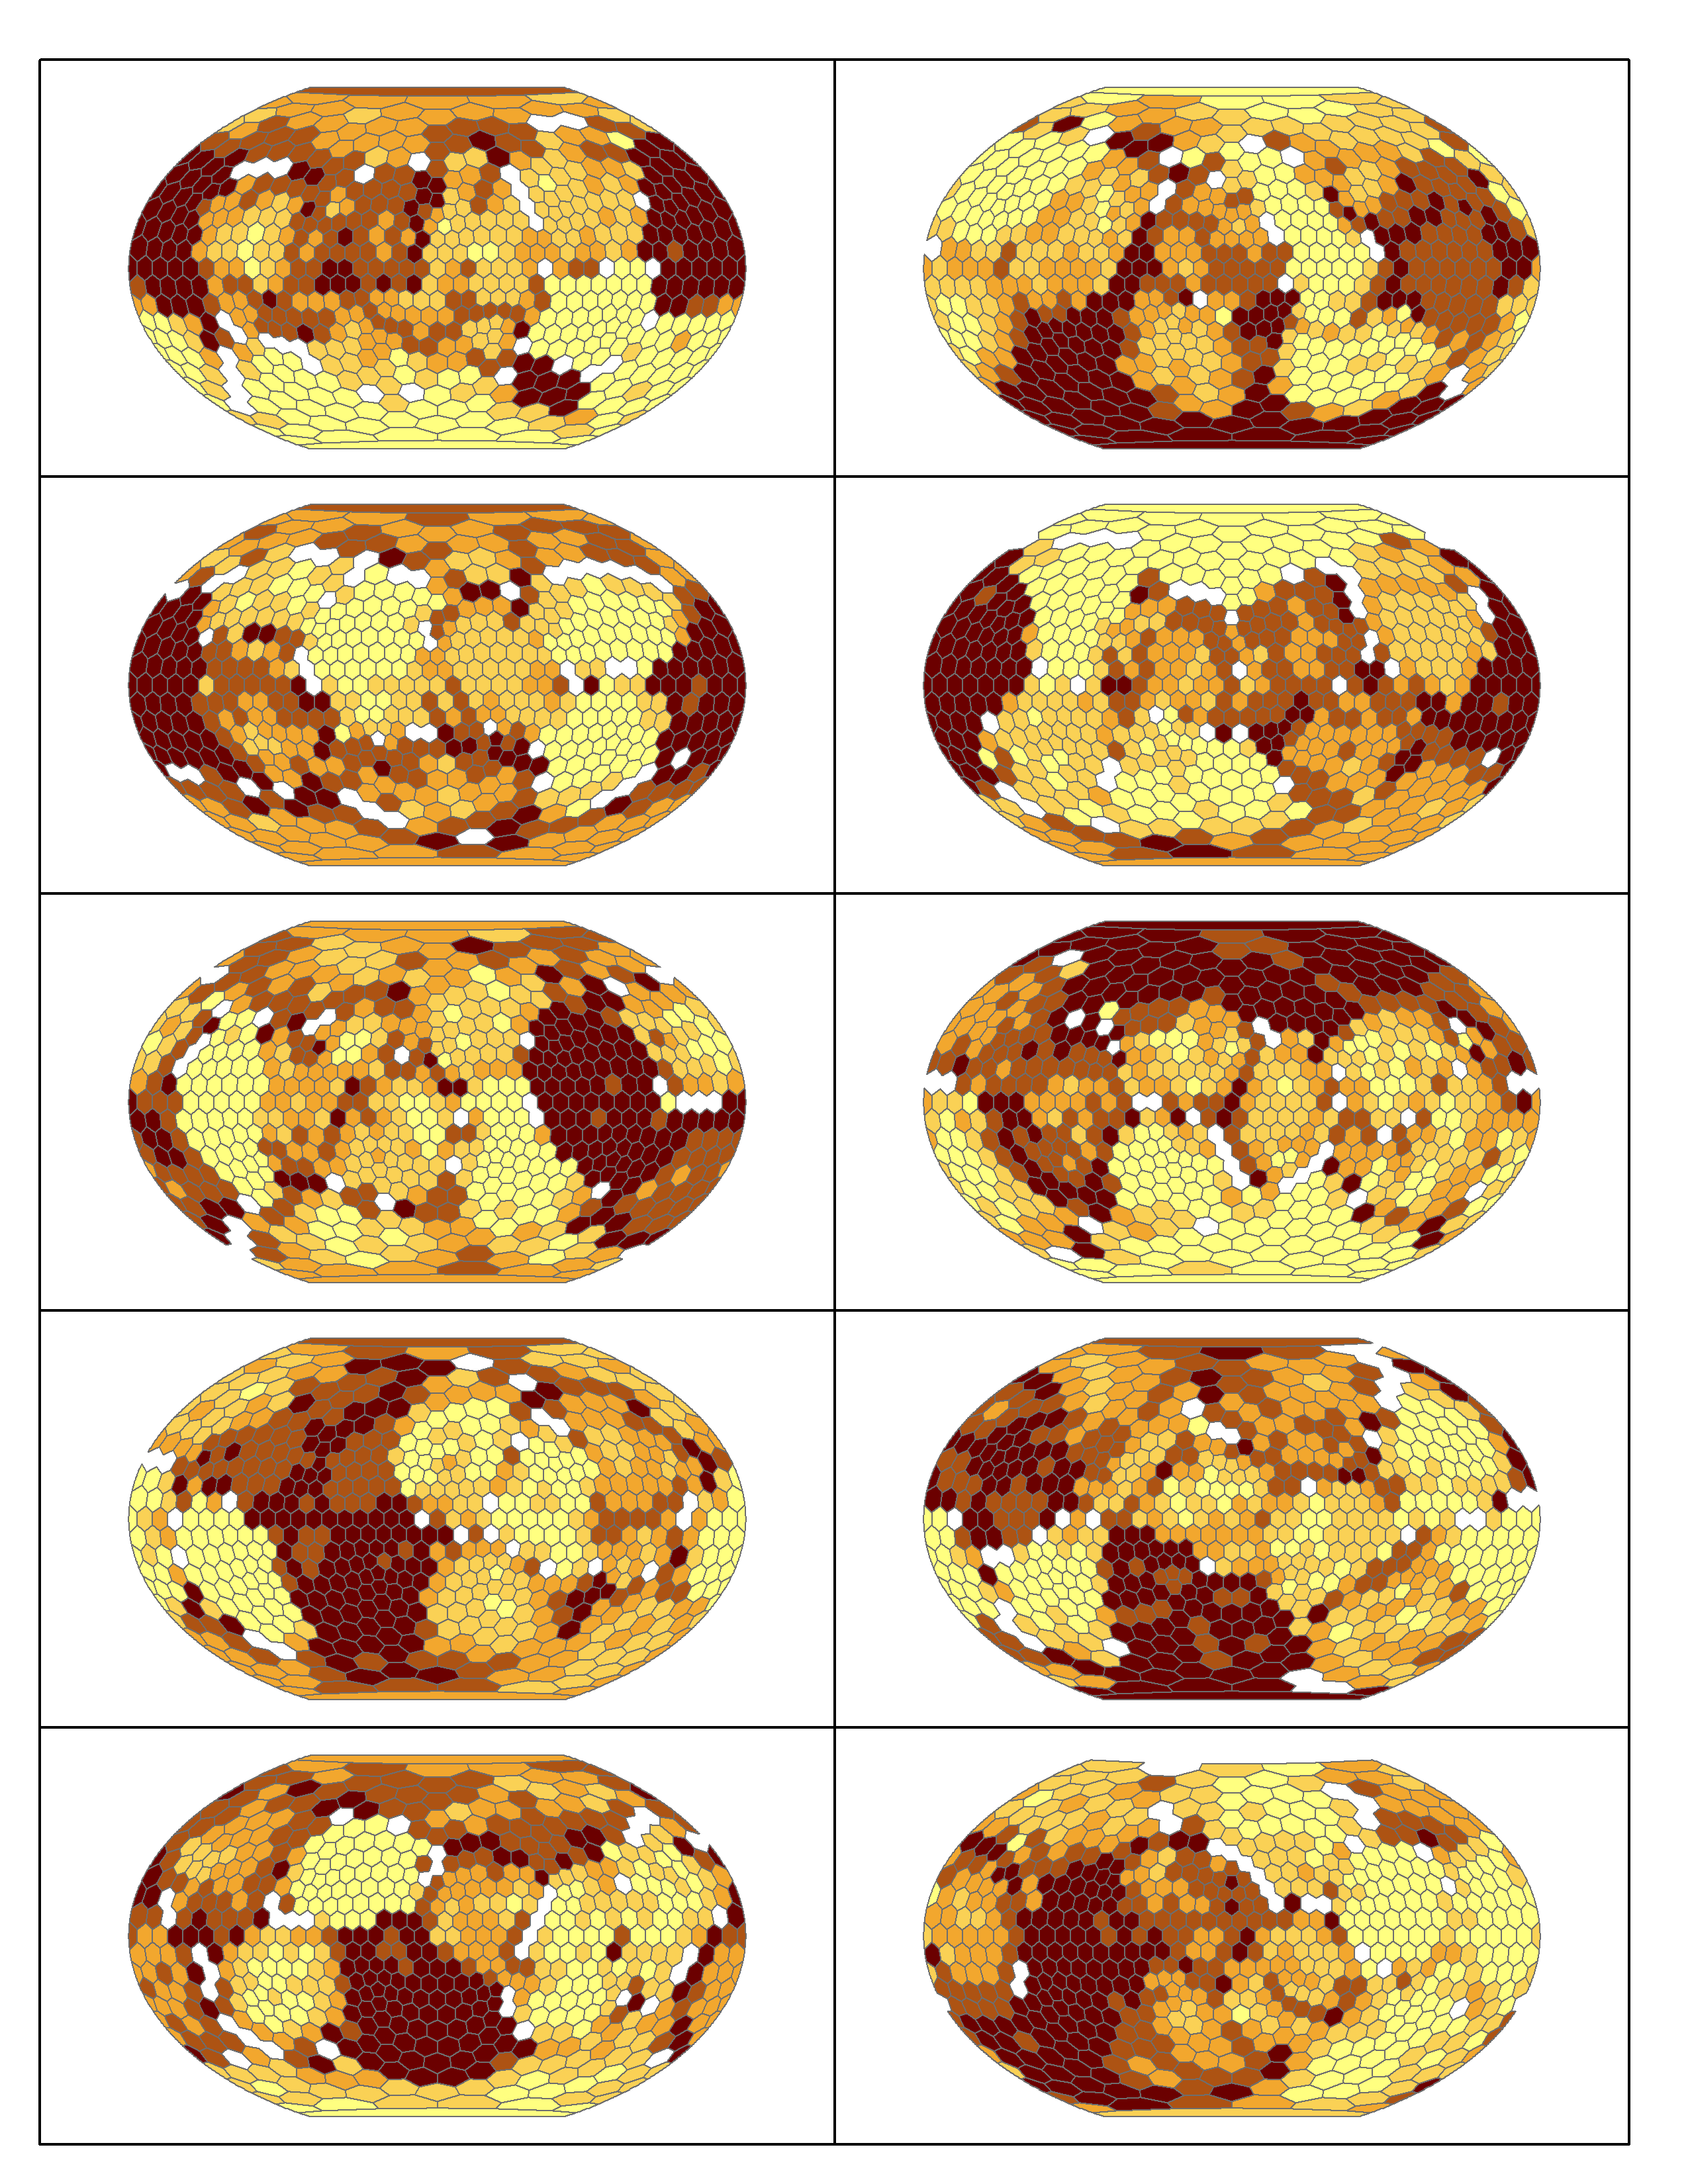
\includegraphics[width=.40\linewidth]{geodesic_winkel.png}
}
\caption{This shows 4 box plots, each representing one group of neurons in a set
of SOMs trained with the same parameters.}
\label{ten}
\end{figure}
